% ============================================================
% v2 RESTRUCTURE (method-paper shape).
%
% NARRATIVE CONTRACT (the plan, documented this time):
%   1. METHOD    -- spec-accept (+ scale-matched loop) is THE
%                   contribution. Not "a study of FF-JEPA".
%   2. CALIBRATE -- tau/k DERIVED by measurement (encoder criterion
%                   floor; sampler convergence point) on the two DEV
%                   envs; validated vs the sweeps; S tuned per env by
%                   a declared rule. (Was "frozen"; upgraded to
%                   "derived" 2026-07-13, 1 prospective hit k=3.)
%   3. EVALUATE  -- recipe applied across PushT, Reacher, + held-out
%                   (Cube: CONFIRMED WIN). The c* arbiter closes the regime
%                   map into a single policy: 4/4 + 5/5 + cube-bar
%                   pre-registered, pooled at 1024 eps/cell, fairness closed
%                   (compute-matched flat, tau-robustness, oracle ceiling,
%                   measured latency). ALL EXPERIMENTAL CLAIMS FINAL
%                   2026-07-16. Remaining TBDs (2): spine cube panel
%                   (plotting), submission-time related-work re-sweep.
%   4. EXPLAIN   -- a dedicated WHY section (mechanism = churn thesis),
%                   because "it wins" is a table; "here is why" is the
%                   paper.
%   5. Reproduction/audit + forensic material -> APPENDIX.
%      Full source for it remains in "paper (1).tex".
%
% Every remaining \tbdblock is a queued experiment or a plotting task.
% ============================================================
\documentclass{article}
\usepackage{iclr2026_conference,times}
\usepackage{graphicx}
\usepackage{amsmath,amssymb}
\usepackage{booktabs}
\usepackage{multirow}
\usepackage{tabularx}
\usepackage{enumitem}
\usepackage{subcaption}
\usepackage{xcolor}
\usepackage{algorithm}
\usepackage{algpseudocode}
\usepackage{tikz}
\usetikzlibrary{arrows.meta,positioning,shapes.geometric,calc}
\usepackage{pgfplots}
\pgfplotsset{compat=1.16}
\definecolor{gapopen}{HTML}{2A78D6}
\definecolor{gapmech}{HTML}{EB6834}
\definecolor{gapdead}{HTML}{E34948}
\usepackage{hyperref}
\usepackage{cleveref}

% ---- house macros ----
\newcommand{\ours}[1]{\textbf{#1}}
\newcommand{\degc}[1]{$#1^\circ$}
\newcommand{\gdm}{\text{GDM}}
\newcommand{\TBD}{\textcolor{red}{\textbf{TBD}}}
\newcommand{\tbdblock}[1]{%
  \begin{center}\fcolorbox{red}{red!5}{%
    \parbox{0.9\linewidth}{\centering\color{red}\textbf{[TBD: #1]}}}%
  \end{center}}
\newcommand{\inflight}[1]{%
  \begin{center}\fcolorbox{orange!70!black}{orange!6}{%
    \parbox{0.9\linewidth}{\small\color{orange!50!black}%
    \textbf{[Pre-registered, in flight]} #1}}%
  \end{center}}

\title{Reality-Verified Speculative Consumption\\
for Hierarchical Latent World-Model Planning}
\author{Anonymous authors \\ Paper under double-blind review}

\begin{document}
\maketitle

\begin{abstract}
When can a drafted subgoal plan be trusted, and for how long? We introduce
\emph{spec-accept}, a training-free consumption rule for hierarchical latent
world-model planners: draft a block of $N$ subgoal latents once, then verify the
achieved latent against the waypoint just pursued at every replan boundary. Within a
relative distance $\tau$, the next pre-drafted waypoint is served at zero drafter
cost; otherwise the block is re-drafted from reality. The verifier is the
environment itself, with no learned components, and both constants are measured
rather than tuned: $\tau$ is the encoder's criterion floor and the step budget $k$
is the sampler's convergence point, each computed offline in minutes. Adding the
planner's own reachability certificate $c^{*}$ yields \emph{certified spec-accept},
which meets or beats the strongest flat baseline in all eleven pre-registered
environment--horizon cells across PushT, Reacher, and held-out Cube, with margins up
to $+94$pp where flat planning collapses, at $1.9$--$2.4$ drafter evaluations per
replan. On the one substrate whose encoder cannot support verification at all
(Two-Room, the LeWM authors' own weakest result), the accept test transplants
unchanged into a frozen external encoder and recovers a $+15.4$pp certified win at
long horizon, at a protocol anchored to the published number; a window rule with its
switch read off the measured crossover composes the two regimes into a policy that
never loses to flat. One mechanism
explains the wins, the ties, and every measured negative:
control pays for target consistency, and re-drafting injects churn proportional to
draft noise. A companion statistic, the verification gap, predicts from cached
latents alone whether a given world model can support the method, and its
predictions have held prospectively on substrates adopted after the rule was frozen.
\end{abstract}

% ============================================================
\section{Introduction}
\label{sec:intro}
Hierarchical latent world models promise long-horizon planning by decomposing a goal
into a chain of reachable subgoals. FF-JEPA \citep{ffjepa} instantiates this on the
LeWM JEPA world model \citep{lewm}: a diffusion model drafts future subgoal latents
and a flat CEM controller \citep{cem} steers toward each in turn, re-planning on a
fixed stride. The system works, hierarchy beats flat planning at long horizon, but two questions go unexamined. It pays one diffusion call at \emph{every} replan,
never asking whether a drafted plan could be \emph{reused} while it still holds; and
it fixes the subgoal spacing to a single value, chosen by convention rather than
matched to anything.

We take the consumption policy as the object of study and ask the method question:
when can a drafted plan be trusted, and for how long? Our answer is to verify against
\emph{reality} rather than a learned critic, in closed-loop control the strongest
possible verifier, the achieved environment state, is free at every replan boundary, and to set the two knobs this introduces by \emph{measurement} rather than search.
Concretely:

\begin{enumerate}[itemsep=2pt,topsep=2pt]
\item \textbf{Spec-accept} (\Cref{sec:method-spec}): a training-free consumption
rule with one threshold and no learned components; it composes with any drafter.
\item \textbf{Calibration by measurement} (\Cref{sec:calib}): $\tau$ and $k$ are
read off two offline measurements in minutes, not swept. The derived PushT $k{=}3$
was a configuration no sweep had run; it was predicted, then confirmed.
\item \textbf{Evaluation and mechanism} (\Cref{sec:results,sec:why}): one frozen
recipe, every comparison anchored to the strongest flat baseline per cell, and one
mechanism (the \emph{churn thesis}) unifying five independent measurements.
\item \textbf{Certified drafting scope}
(\Cref{sec:method-arbiter,sec:results-unified}): the planner's own certificate
$c^{*}$ routes each episode to flat planning or drafting and retires the drafter on
certified arrival, producing one policy that wins all eleven pre-registered cells.
\item \textbf{Verifier modularity} (\Cref{sec:results-heldout}): when the gap
statistic rules the planner's own space out (Two-Room), the accept test transplants
unchanged into a frozen external encoder; the certified loop then beats flat by
$+15.4$pp at long horizon at a protocol anchored to LeWM's published number, and the
window rule composes flat and certified drafting into a policy that never loses,
with the crossover confirmed where it was predicted.
\item \textbf{Honest scope} (\Cref{sec:discussion}): every boundary of the
derivation is measured and reported, alongside a battery of negative results that
causally implicate drafter stochasticity.
\end{enumerate}

% ============================================================
\section{Related Work}
\label{sec:related}

\paragraph{Latent world models and planning.} LeWM \citep{lewm} plans with CEM
\citep{cem} over a frozen JEPA latent space; DINO-WM \citep{dinowm} and PLDM
\citep{pldm} take the same frozen-encoder, latent-dynamics route. FF-JEPA
\citep{ffjepa} adds a diffusion subgoal drafter on top of LeWM and is our substrate;
we modify only its subgoal scale, loop matching, and consumption policy.

\paragraph{Hierarchical and diffusion-based planning.} Trajectory-level diffusion
planners \citep{janner2022diffuser} and their hierarchical variants
\citep{chen2024hierarchical} draft subgoals or waypoint sequences for a low-level
controller. Across this line the subgoal spacing is a design constant fixed by
convention; we treat it as the dominant lever, tune it in the open, and report its
behavior (an interior optimum, matched to the control loop) as a finding.

\paragraph{Speculative decoding.} Draft--verify--accept decoding
\citep{leviathan2023fast,chen2023accelerating} accelerates autoregressive generation
with a cheap drafter and an exact verifier. DSpark \citep{dspark} schedules
commitment with a learned confidence head over semi-autoregressive drafts; ported
literally to latent control, every learned component hurts (\Cref{sec:negatives}), the skeleton survives only once the learned verifier is replaced by the achieved
environment state. The distinction is structural: in language there is no environment
to consult mid-generation; in closed-loop control the strongest possible verifier is
free at every replan boundary.

\paragraph{Commitment and chunking in control.} Action-chunking policies face the
same trust question one level down: how long to follow a committed open-loop segment.
Bidirectional decoding \citep{bid} rejection-samples chunks under backward-coherence
and forward-contrast criteria; real-time chunking \citep{rtc} manages chunk
continuation under asynchronous inference; training-free chunk correction
\citep{dcdp} injects dynamic features into a pretrained diffusion policy. These
operate on \emph{actions} with learned or heuristic critics; spec-accept verifies
\emph{plan adherence} in latent state space against reality itself, with one
threshold and no new parameters. Concurrently, speculative policy orchestration
\citep{spo} speculatively executes cloud policy outputs to mask network latency, speculation over transport, not over drafter compute.

\paragraph{Few-step diffusion.} DDIM \citep{ddim} and consistency-style few-step
samplers \citep{consistency} make individual diffusion calls cheap; our $k{=}50\to4$
result is this factor applied to subgoal drafting, and the paper keeps it separated
from verified consumption (spec-accept's own contribution) throughout.

% Concurrent-work sweep last re-run 2026-07-27: SAGE (arXiv 2607.17973, concurrent
% subgoal drafting on LeWM; cited as premise validation, differentiated on
% certification -- protocols not cross-comparable) and TRM (arXiv 2605.22164,
% lens-adjacent metric repair) folded into the paragraphs above. Re-check once at
% camera-ready.

% ============================================================
\section{Background: The Hierarchical Latent Planner}
\label{sec:setup}
The substrate is the FF-JEPA stack: a frozen LeWM JEPA (ViT encoder + latent
dynamics), a diffusion subgoal drafter (``\gdm{}'', DiT, ${\sim}53$M params) proposing
blocks of $N{=}3$ future latents spaced $S$ steps apart, and a CEM controller planning
action blocks of 5 steps toward the current latent target with receding horizon RH.
Goals are hindsight frames $t$ steps ahead; success is each benchmark's shipped
criterion. All results are produced by a pipeline rebuilt end-to-end from public
assets; its closed-loop anchor cells reproduce the original system's numbers within
noise (\Cref{app:repro}); per-environment protocols are tabulated in
\Cref{tab:protocols}.

\paragraph{Statistical conventions and scope.} Every quoted cell pools $64$--$128$
episodes per seed over $4$--$12$ evaluation seeds ($384$--$1536$ episodes; grid
confirmations at $1024$/cell), with margins tested paired per-seed wherever seeds
match. For calibration, the substrate's own paper \citep{lewm} evaluates $50$
trajectories per published bar and reports training-seed variance ($3$ retrainings)
for one environment; in the single place that convention binds, the Two-Room anchor
replication, we ran their protocol verbatim \emph{including} $n{=}50$.\footnote{One
released-vs-text discrepancy, resolved in the data's favor: their paper text states
$10$ CEM iterations outside PushT while their released configuration specifies $30$;
we follow the released configuration, which is the one that reproduces their
published Two-Room number.} Our seeds are \emph{evaluation} seeds (episode sampling
and CEM) on the frozen released checkpoint: substrate training variance is
deliberately out of scope, since the method takes the stack as given and the
released weights are what makes anchor comparisons faithful. Generality beyond this
checkpoint is tested on a stronger axis instead, across architectures
(\Cref{sec:generality}).

% ============================================================
\section{Method}
\label{sec:method}

\subsection{Reality-verified speculative consumption (spec-accept)}
\label{sec:method-spec}
Every-step drafting pays one diffusion call per replan. Spec-accept drafts a block of
$N$ waypoints once, then at each replan boundary verifies \emph{reality} against the
plan: if the achieved latent is within relative distance $\tau$ of the waypoint just
pursued, the next pre-drafted waypoint is served at zero drafter cost; otherwise the
block is re-drafted from the achieved state. Re-anchoring is never sacrificed, drafting is skipped only while reality confirms the plan. The verifier is the
environment itself: no learned confidence head, no schedule, no new parameters, and it
composes with any drafter.

\begin{algorithm}[h]
\small
\caption{Spec-accept: reality-verified speculative consumption (one env; run per env).}
\label{alg:specaccept}
\begin{algorithmic}[1]
\Require frozen encoder $E$, drafter $G$ (block size $N$, $k$ DDIM steps), controller
CEM, threshold $\tau$; horizon RH$\,{=}\,S/5$
\State $\mathrm{block}\gets G(E(o_0);\,k)$;\quad $j\gets 1$;\quad $w\gets \mathrm{block}[0]$
\Comment{initial draft; $j$ indexes the served position}
\For{each replan boundary with achieved observation $o$}
  \State $z\gets E(o)$
  \If{$j<N$ \textbf{and} $\|z-w\|/\|z\| \le \tau$}
     \Comment{reality confirms the plan, accept, no diffusion call}
     \State $w\gets \mathrm{block}[j]$;\quad $j\gets j+1$
  \Else
     \Comment{reality diverged (or block exhausted), re-anchor}
     \State $\mathrm{block}\gets G(z;\,k)$;\quad $w\gets \mathrm{block}[0]$;\quad $j\gets 1$
  \EndIf
  \State execute CEM toward $w$ for RH action blocks
\EndFor
\end{algorithmic}
\end{algorithm}

% Figure: the certified spec-accept loop (TikZ). Input from main via
% % Figure: the certified spec-accept loop (TikZ). Input from main via
% % Figure: the certified spec-accept loop (TikZ). Input from main via
% \input{figures/fig_method_tikz}. Requires tikz + libraries loaded in preamble:
% \usetikzlibrary{arrows.meta,positioning,shapes.geometric,calc}
\begin{figure}[t]
\centering
\resizebox{0.86\linewidth}{!}{%
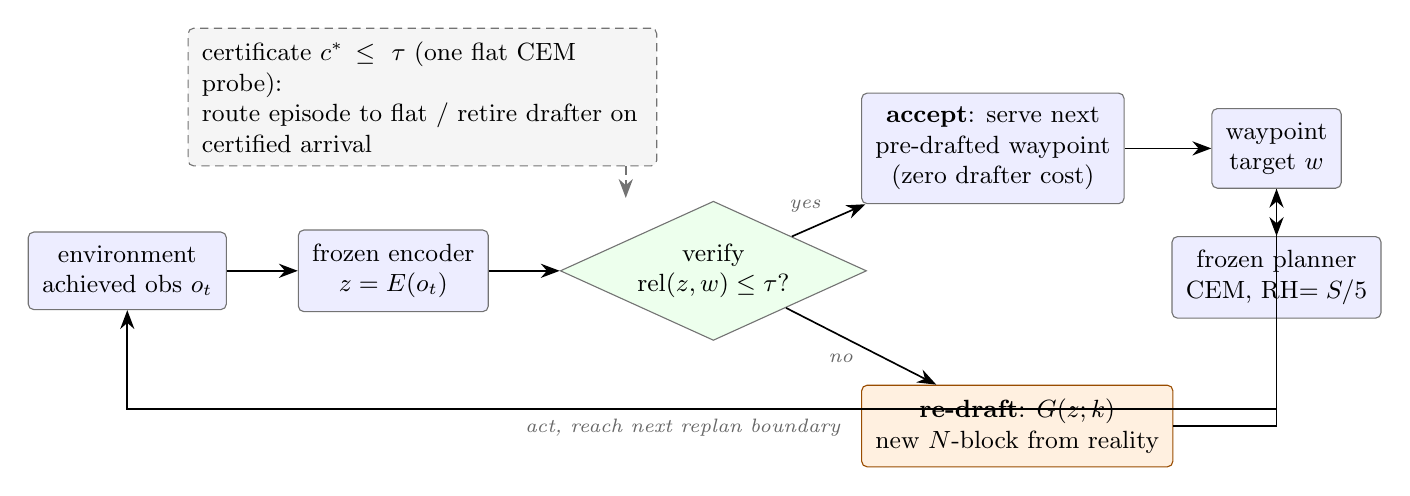
\begin{tikzpicture}[
  font=\small,
  node distance=6mm and 9mm,
  box/.style={draw=black!55, rounded corners=2pt, align=center,
              inner sep=5pt, minimum height=8mm},
  frozen/.style={box, fill=blue!7},
  paid/.style={box, fill=orange!12, draw=orange!60!black},
  verify/.style={diamond, draw=black!55, fill=green!7, align=center,
                 inner sep=2pt, aspect=2.2},
  cert/.style={box, fill=black!4, densely dashed},
  arr/.style={-{Stealth[length=2.4mm]}, semithick},
  lbl/.style={font=\scriptsize\itshape, text=black!60},
]
% main loop
\node[frozen] (env) {environment\\achieved obs $o_t$};
\node[frozen, right=of env] (enc) {frozen encoder\\$z=E(o_t)$};
\node[verify, right=of enc] (ver) {verify\\$\mathrm{rel}(z,w)\le\tau$?};
\node[frozen, above right=4mm and 9mm of ver] (accept)
  {\textbf{accept}: serve next\\pre-drafted waypoint\\(zero drafter cost)};
\node[paid, below right=10mm and 9mm of ver] (draft)
  {\textbf{re-draft}: $G(z;k)$\\new $N$-block from reality};
\node[frozen, right=of accept, xshift=2mm] (target) {waypoint\\target $w$};
\node[frozen, below=of target] (cem) {frozen planner\\CEM, RH$=S/5$};

\draw[arr] (env) -- (enc);
\draw[arr] (enc) -- (ver);
\draw[arr] (ver) -- node[lbl, above left=-1pt]{yes} (accept);
\draw[arr] (ver) -- node[lbl, below left=-1pt]{no} (draft);
\draw[arr] (accept) -- (target);
\draw[arr] (draft) -| (target);
\draw[arr] (target) -- (cem);
\draw[arr] (cem.south) |- ++(-2.0,-1.15) -| node[lbl, pos=0.22, below]{act, reach next replan boundary} (env.south);

% certificate rail (kept clear of the accept node: anchored over env/enc only)
\node[cert, above=8mm of enc.north west, anchor=south west, xshift=-14mm,
      text width=5.6cm, align=left] (cstar)
  {certificate $c^{*}\!\le\tau$ (one flat CEM probe):\\
   route episode to flat / retire drafter on\\certified arrival};
\draw[arr, densely dashed, black!55] (cstar.south east) ++(-4mm,0) -- ++(0,-4mm);
\end{tikzpicture}%
}
\caption{\textbf{Certified spec-accept.} A drafted $N$-block is consumed waypoint by
waypoint; at every replan boundary the \emph{achieved} latent is verified against
the waypoint just pursued. Within $\tau$, the next pre-drafted waypoint is served
at zero drafter cost; otherwise the block is re-drafted from reality. Encoder,
planner, and world model stay frozen (blue); the drafter (orange) is the only paid
component, and the planner's own certificate $c^{*}$ (dashed) decides per episode
and per replan whether drafting is needed at all. $\tau$ is derived, not tuned
(\Cref{sec:calib-tau}).}
\label{fig:method}
\end{figure}
. Requires tikz + libraries loaded in preamble:
% \usetikzlibrary{arrows.meta,positioning,shapes.geometric,calc}
\begin{figure}[t]
\centering
\resizebox{0.86\linewidth}{!}{%
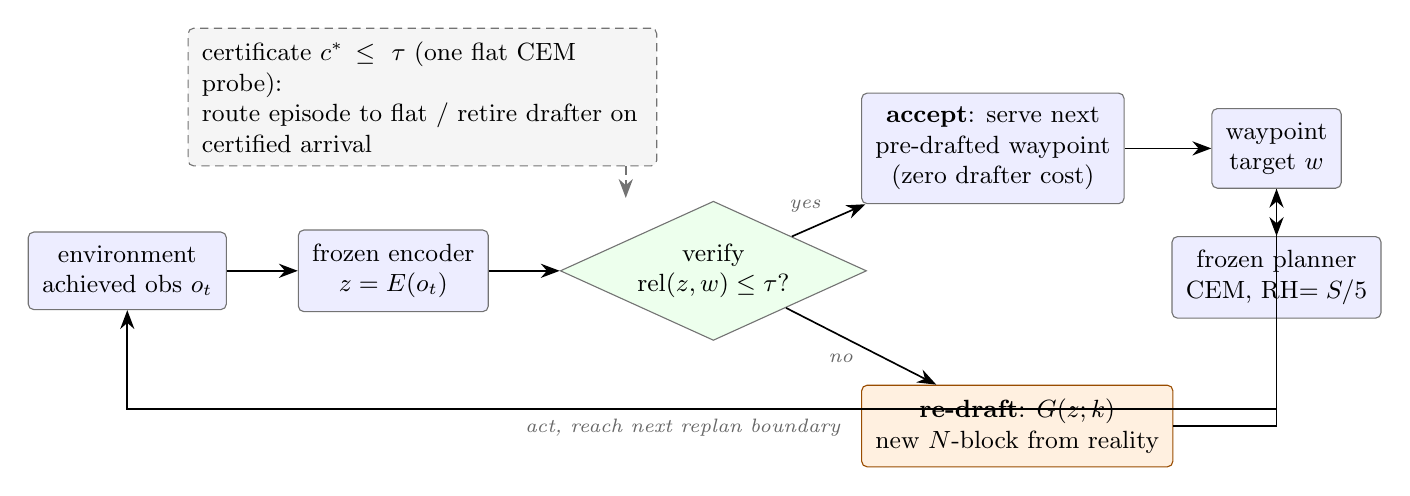
\begin{tikzpicture}[
  font=\small,
  node distance=6mm and 9mm,
  box/.style={draw=black!55, rounded corners=2pt, align=center,
              inner sep=5pt, minimum height=8mm},
  frozen/.style={box, fill=blue!7},
  paid/.style={box, fill=orange!12, draw=orange!60!black},
  verify/.style={diamond, draw=black!55, fill=green!7, align=center,
                 inner sep=2pt, aspect=2.2},
  cert/.style={box, fill=black!4, densely dashed},
  arr/.style={-{Stealth[length=2.4mm]}, semithick},
  lbl/.style={font=\scriptsize\itshape, text=black!60},
]
% main loop
\node[frozen] (env) {environment\\achieved obs $o_t$};
\node[frozen, right=of env] (enc) {frozen encoder\\$z=E(o_t)$};
\node[verify, right=of enc] (ver) {verify\\$\mathrm{rel}(z,w)\le\tau$?};
\node[frozen, above right=4mm and 9mm of ver] (accept)
  {\textbf{accept}: serve next\\pre-drafted waypoint\\(zero drafter cost)};
\node[paid, below right=10mm and 9mm of ver] (draft)
  {\textbf{re-draft}: $G(z;k)$\\new $N$-block from reality};
\node[frozen, right=of accept, xshift=2mm] (target) {waypoint\\target $w$};
\node[frozen, below=of target] (cem) {frozen planner\\CEM, RH$=S/5$};

\draw[arr] (env) -- (enc);
\draw[arr] (enc) -- (ver);
\draw[arr] (ver) -- node[lbl, above left=-1pt]{yes} (accept);
\draw[arr] (ver) -- node[lbl, below left=-1pt]{no} (draft);
\draw[arr] (accept) -- (target);
\draw[arr] (draft) -| (target);
\draw[arr] (target) -- (cem);
\draw[arr] (cem.south) |- ++(-2.0,-1.15) -| node[lbl, pos=0.22, below]{act, reach next replan boundary} (env.south);

% certificate rail (kept clear of the accept node: anchored over env/enc only)
\node[cert, above=8mm of enc.north west, anchor=south west, xshift=-14mm,
      text width=5.6cm, align=left] (cstar)
  {certificate $c^{*}\!\le\tau$ (one flat CEM probe):\\
   route episode to flat / retire drafter on\\certified arrival};
\draw[arr, densely dashed, black!55] (cstar.south east) ++(-4mm,0) -- ++(0,-4mm);
\end{tikzpicture}%
}
\caption{\textbf{Certified spec-accept.} A drafted $N$-block is consumed waypoint by
waypoint; at every replan boundary the \emph{achieved} latent is verified against
the waypoint just pursued. Within $\tau$, the next pre-drafted waypoint is served
at zero drafter cost; otherwise the block is re-drafted from reality. Encoder,
planner, and world model stay frozen (blue); the drafter (orange) is the only paid
component, and the planner's own certificate $c^{*}$ (dashed) decides per episode
and per replan whether drafting is needed at all. $\tau$ is derived, not tuned
(\Cref{sec:calib-tau}).}
\label{fig:method}
\end{figure}
. Requires tikz + libraries loaded in preamble:
% \usetikzlibrary{arrows.meta,positioning,shapes.geometric,calc}
\begin{figure}[t]
\centering
\resizebox{0.86\linewidth}{!}{%
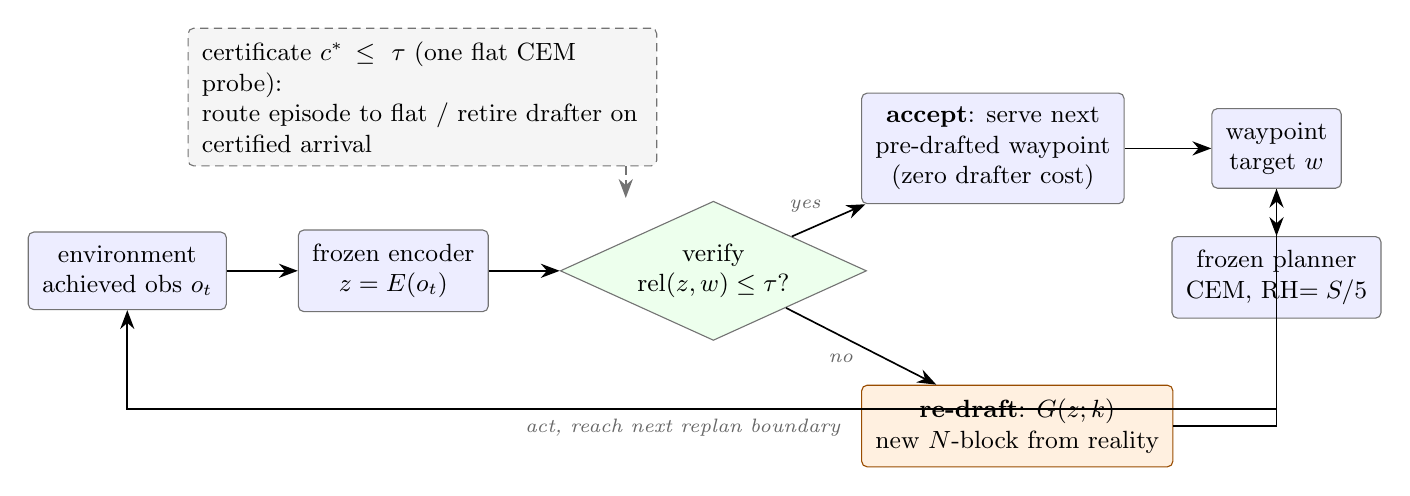
\begin{tikzpicture}[
  font=\small,
  node distance=6mm and 9mm,
  box/.style={draw=black!55, rounded corners=2pt, align=center,
              inner sep=5pt, minimum height=8mm},
  frozen/.style={box, fill=blue!7},
  paid/.style={box, fill=orange!12, draw=orange!60!black},
  verify/.style={diamond, draw=black!55, fill=green!7, align=center,
                 inner sep=2pt, aspect=2.2},
  cert/.style={box, fill=black!4, densely dashed},
  arr/.style={-{Stealth[length=2.4mm]}, semithick},
  lbl/.style={font=\scriptsize\itshape, text=black!60},
]
% main loop
\node[frozen] (env) {environment\\achieved obs $o_t$};
\node[frozen, right=of env] (enc) {frozen encoder\\$z=E(o_t)$};
\node[verify, right=of enc] (ver) {verify\\$\mathrm{rel}(z,w)\le\tau$?};
\node[frozen, above right=4mm and 9mm of ver] (accept)
  {\textbf{accept}: serve next\\pre-drafted waypoint\\(zero drafter cost)};
\node[paid, below right=10mm and 9mm of ver] (draft)
  {\textbf{re-draft}: $G(z;k)$\\new $N$-block from reality};
\node[frozen, right=of accept, xshift=2mm] (target) {waypoint\\target $w$};
\node[frozen, below=of target] (cem) {frozen planner\\CEM, RH$=S/5$};

\draw[arr] (env) -- (enc);
\draw[arr] (enc) -- (ver);
\draw[arr] (ver) -- node[lbl, above left=-1pt]{yes} (accept);
\draw[arr] (ver) -- node[lbl, below left=-1pt]{no} (draft);
\draw[arr] (accept) -- (target);
\draw[arr] (draft) -| (target);
\draw[arr] (target) -- (cem);
\draw[arr] (cem.south) |- ++(-2.0,-1.15) -| node[lbl, pos=0.22, below]{act, reach next replan boundary} (env.south);

% certificate rail (kept clear of the accept node: anchored over env/enc only)
\node[cert, above=8mm of enc.north west, anchor=south west, xshift=-14mm,
      text width=5.6cm, align=left] (cstar)
  {certificate $c^{*}\!\le\tau$ (one flat CEM probe):\\
   route episode to flat / retire drafter on\\certified arrival};
\draw[arr, densely dashed, black!55] (cstar.south east) ++(-4mm,0) -- ++(0,-4mm);
\end{tikzpicture}%
}
\caption{\textbf{Certified spec-accept.} A drafted $N$-block is consumed waypoint by
waypoint; at every replan boundary the \emph{achieved} latent is verified against
the waypoint just pursued. Within $\tau$, the next pre-drafted waypoint is served
at zero drafter cost; otherwise the block is re-drafted from reality. Encoder,
planner, and world model stay frozen (blue); the drafter (orange) is the only paid
component, and the planner's own certificate $c^{*}$ (dashed) decides per episode
and per replan whether drafting is needed at all. $\tau$ is derived, not tuned
(\Cref{sec:calib-tau}).}
\label{fig:method}
\end{figure}


\noindent $\tau{\to}0$ recovers every-step drafting (re-draft always); $\tau{\to}\infty$
recovers blind commitment (consume the whole block, never check). The realized fraction
of boundaries that re-draft is the \emph{call ratio}, reported throughout as
spec-accept's own cost factor and, per episode, as a free diagnostic of how often
reality is leaving the plan.

\subsection{Scale matching: the control loop follows the subgoal spacing}
\label{sec:method-scale}
The drafter's subgoal spacing $S$ is the recipe's one per-environment quantity, and the
controller is matched to it; RH $= S/5$ action blocks per replan; so a drafted
waypoint is consumed exactly when the planner has had the lookahead to reach it.
Mismatching them is not a detail: re-anchoring every 5 steps against unchanged
25-step targets \emph{collapses} SR by $12$pp (cadence-isolation control,
\Cref{app:controls}), the mechanism is scale matching, not replanning frequency.

\subsection{Calibration protocol: two knobs measured, one tuned}
\label{sec:method-config}
$\tau$ and $k$ are not tuned: each is \emph{derived} from an offline measurement of
the stack (\Cref{sec:calib}), computed in minutes with no closed-loop rollouts, and
the closed-loop sweeps we also ran serve as validation of the derivation rather than
as the selection mechanism. $S$ is the one tuned knob, and its behavior is reported
as a finding. Held-out environments (\Cref{sec:results-heldout}) receive the recipe
derive-first: $\tau$ and $k$ are computed from the new environment's encoder and
drafter and pre-registered before any closed-loop cell is run.

\begin{table}[h]
\centering
\small
\caption{Configuration policy. $\tau$ and $k$ are measured properties of the stack;
$S$ is tuned and reported as a result.}
\label{tab:config}
\begin{tabular}{llp{8.2cm}}
\toprule
knob & value (dev envs) & basis \\
\midrule
$\tau$ (acceptance threshold) & $0.20$ & \emph{derived}: the encoder's criterion
floor, the latent distance at which the benchmark's own success tolerance stops
distinguishing states (\Cref{sec:calib-tau}); validated retrospectively against
closed-loop grids on both dev environments and an episode-disjoint split \\
$k$ (DDIM steps per draft) & $3$ (PushT) / any (Reacher) & \emph{derived}: the
sampler's convergence point, measured by repeat-draw dispersion
(\Cref{sec:calib-k}); on PushT the derived $k{=}3$ was never swept and was confirmed
prospectively; the inherited $k{=}50$ is image-domain convention,
${\sim}17\times$ overpriced \\
$S$ (subgoal scale) & per env, tuned & swept on dev envs; both show an interior
optimum at $S{=}10$ at short range (\Cref{sec:calib-scale}). Pre-registered rule for
held-out envs: $S{=}10$ zero-shot as the primary arm (transfer of the dev-env
optimum), gated by an offline displacement sanity probe ($\mathrm{disp}(S)$ well
above the criterion floor); an optional $S\in\{5,25\}$ secondary curve is reported
as a finding, never used for selection \\
$\gamma$ (draft noise scale) & $1$ (native) & not a knob: swept once as a mechanism
experiment (\Cref{sec:why}) \\
\bottomrule
\end{tabular}
\end{table}

One-knob-at-a-time sweeping is licensed by measured $\tau{\times}k$ separability (full
cross-grid on Reacher; off-axis spot-check on PushT). The cost claim is always stated
as two separable factors: \emph{cheap drafts} ($k{=}50{\to}3$/$4$, available to
every-step drafting too) $\times$ \emph{verified consumption} (spec-accept's own
call reduction at matched $k$, ratios $0.5$--$0.8$, SR-neutral).

\subsection{Certified drafting scope: the $c^{*}$ arbiter}
\label{sec:method-arbiter}
Drafting is conditional (\Cref{sec:why-regime}): where the goal is already inside the
planner's lookahead, even ground-truth waypoints do not beat flat planning, and drafted
ones actively lose. Rather than leave that as a per-task caveat, we make the policy
decide it, using the planner's own machinery, and no new threshold. Before
committing to anything, run one \emph{flat} CEM plan from the achieved latent toward
the goal latent, the exact plan the flat baseline would execute, and read its
predicted terminal discrepancy under the world model,
\[
c^{*} \;=\; \mathrm{rel}\!\left(\hat z_{H},\, z_{\mathrm{goal}}\right)
\;=\; \frac{\lVert \hat z_{H}-z_{\mathrm{goal}}\rVert}{\lVert \hat z_{H}\rVert},
\]
the planner's self-assessment of how close its best direct plan will land. The
arbitration rule, applied at two scopes with the verifier's own $\tau$:

\begin{itemize}[itemsep=1pt,topsep=2pt]
\item \textbf{Episode scope (routing).} At the first replan, if $c^{*}\!\le\tau$ under
the short planning window the episode runs flat at that window; else, if $c^{*}\!\le\tau$
under the deep window (RH$=$5), it runs flat at the deep window; otherwise it drafts
(spec-accept). One decision per episode, from the start state only.
\item \textbf{Replan scope (retirement).} Inside a drafting episode, $c^{*}$ is
re-read at each replan; the first time it crosses $\tau$, the goal has come inside
the planner's own window, the drafter \emph{retires}, one-way, and the goal latent
is served directly thereafter (zero further drafter calls).
\end{itemize}

The two scopes are one rule at two granularities, the episode-start check
\emph{is} the first retirement check, and together they define \emph{certified
spec-accept}, the single method this paper evaluates; the results additionally
report a routing-only ablation (retirement disabled) to isolate each scope's
contribution (\Cref{tab:unified}). $c^{*}$ never firing recovers plain spec-accept
exactly; always firing recovers flat planning: certified spec-accept interpolates
between its parents per episode, chosen by the planner's certificate rather than by
us. Three properties matter. (i)
\emph{No new constants}: the threshold is the verifier's $\tau$, third use, never
re-tuned. (ii) \emph{The certificate and the execution cannot disagree by
construction}: $c^{*}$ is computed by the same solver, cost, and dynamics that will
execute the plan, which is why its per-episode selection is nearly pure in practice
(the episodes it routes to flat succeed at $96$--$100\%$ even at horizons where flat's
population average is $60\%$; \Cref{sec:results-unified}). (iii) \emph{Cost
asymmetry}: routed-to-flat and retired episodes make zero drafter calls; drafting
episodes pay one extra flat CEM solve per replan (measured $1.6\times$ baseline
wall-clock, \Cref{sec:results-eff}). We considered gating on raw latent distance to
the goal instead, it is cheaper, but encoder distances saturate beyond one hop
(\Cref{sec:calib-tau}) and the resulting gate destroys the long-horizon advantage it
is meant to protect (\Cref{sec:negatives}); the planner's certificate is the
instrument that carries per-episode signal at every horizon.

% ============================================================
\section{Calibration by Measurement}
\label{sec:calib}
% Derivation-first: each knob gets (i) the offline measurement that names it,
% (ii) the closed-loop sweeps as VALIDATION, (iii) the honest evidence tier.
The accept test operates in one unit: the relative latent distance
$\mathrm{rel}(a,b) = \|a-b\|/\|a\|$ between the achieved latent and the waypoint
pursued. Both calibration measurements are computed in this same unit, offline, with
no closed-loop rollouts (one GPU, minutes per environment; the probe script is
released), and drop into the controller unconverted.

\subsection{$\tau$ is the encoder's criterion floor}
\label{sec:calib-tau}
Two states can differ in latent space while being the same situation under the
benchmark's own success test, the encoder has finite resolution relative to the
task tolerance. We measure it directly: sample pairs of frames from
\emph{different} episodes whose ground-truth states are equivalent under the
benchmark's success criterion (PushT: agent$+$block position within $20$px, angle
within \degc{20}; Reacher: all joints within $0.05$\,rad), encode both, and record
$\mathrm{rel}$. The distribution of these distances is the \textbf{criterion floor}:
below it, a latent discrepancy carries no task information, so a verifier that
rejects there is re-drafting on noise; far above it, real divergence is being
accepted. The threshold is therefore the floor itself.

\begin{table}[h]
\centering
\small
\caption{The floor measurements (accept-test units, $n{=}436$--$512$ pairs/anchors).
Derived $\tau$ = the criterion floor; the value used everywhere in this paper
($0.20$) sits on both environments' floors, and the environments' \emph{different}
floors predict their different closed-loop plateaus (\Cref{tab:taugrid}).}
\label{tab:floor}
\begin{tabular}{lcccc}
\toprule
& \multicolumn{2}{c}{PushT} & \multicolumn{2}{c}{Reacher} \\
\cmidrule(lr){2-3}\cmidrule(lr){4-5}
& p50 & p90 & p50 & p90 \\
\midrule
temporal floor (consecutive frames)     & 0.080 & 0.152 & 0.223 & 0.428 \\
criterion floor (success-equivalent)    & 0.233 & 0.843 & 0.106 & 0.153 \\
criterion floor, strict (\degc{5})      & 0.173 & 0.718 & ---   & ---   \\
\midrule
reference: true $S{=}10$ displacement   & 0.700 & 1.085 & 0.866 & 1.351 \\
\bottomrule
\end{tabular}
\end{table}

\paragraph{Validation against the closed loop.} The sweeps of \Cref{tab:taugrid}
were run independently and agree with the measurement three ways. (i) Both
environments' swept optima sit on their measured floors ($0.20$ vs.\ PushT's
$0.17$--$0.23$; $0.20$ at the top of Reacher's $0.11$--$0.15$ band). (ii) The
\emph{cross-environment shape} follows the floors; Reacher's lower floor predicts
its plateau ends earlier, and it does (degrades at $\tau{=}0.3$, collapses at $0.4$)
while PushT, with the higher floor, is still flat at $0.3$. (iii) Below the floor the
false-reject signature appears on both environments: tightening $\tau$ from $0.2$ to
$0.1$ buys ${\sim}35\%$ more drafter calls and zero SR. (iv) A \emph{prospective}
corollary test: the band's upper edge should scale with the real-divergence scale, coarser $S$ means larger per-hop tracking error, so looser $\tau$ should stay
in-band exactly there. Registered and then run at $S{=}25$ ($t{=}100$, 4 seeds):
$\tau{=}0.4$ matches $\tau{=}0.2$'s SR ($64.2{\pm}1.4$ vs.\ $63.2{\pm}0.4$) at
$27\%$ fewer calls (ratio $0.64$ vs.\ $0.88$), while the same $\tau{=}0.4$ degrades
$5$pp at the $S{=}10$-scale Reacher setting, the band widens with $S$, as
predicted (and as the earliest offline calibration had hinted). Evidence tier,
stated plainly: checks (i)--(iii) are retrospective (the sweeps predated the
measurement); check (iv) and the $k{=}3$ cell (\Cref{sec:calib-k}) are prospective;
the held-out environments of \Cref{sec:results-heldout} are the pre-registered
derive-first test.

\begin{table}[h]
\centering
\small
\caption{Closed-loop $\tau$-grids, the \emph{validation} of the derived threshold
(\degc{20} / joint criterion; call ratio in parentheses). PushT anchors on the
unfiltered (harder) fixed populations; Reacher on the max-offset-100 fixed
population; $n{=}512$/cell except val split ($n{=}512$, 2 seeds). SR flat inside
each environment's floor band, calls monotone, degradation onset ordered by the
floors (\Cref{tab:floor}).}
\label{tab:taugrid}
\begin{tabular}{lcccccc}
\toprule
& $\tau{=}0.10$ & $0.15$ & $0.20$ & $0.25$ & $0.30$ & $0.40$ \\
\midrule
PushT $t{=}100$, $k{=}4$        & 64.1 (.87) & --- & 65.0 (.58) & --- & 65.0 (.47) & --- \\
PushT val split $t{=}150$, $k{=}8$ & --- & 63.5 (.61) & 64.5 (.50) & 63.7 (.45) & 63.7 (.42) & --- \\
Reacher $t{=}100$, $k{=}4$      & 95.9 (.84) & --- & 95.5 (.63) & --- & 94.1 (.52) & 90.2 (.46) \\
\bottomrule
\end{tabular}
\end{table}

\subsection{$k$ is the sampler's convergence point}
\label{sec:calib-k}
Cheap drafts are consumable only once the sampler has \emph{converged}: repeated
draws from identical conditioning must be versions of the same plan, not partially
denoised noise. We measure this directly: $8$ repeat-draws of the position-1
waypoint at each $k\in\{1,2,3,4,5,6,8,12,16,50\}$, recording per-draw dispersion and
the distance of each $k$'s mean to the converged ($k{=}50$) mean, in accept-test
units. On PushT the transition is not gradual but a step: at $k{=}2$ draws are
unrelated to the converged answer (bias $1.04$, dispersion $0.65$); at $k{=}3$ they
snap into place (bias $0.11$, dispersion $0.080$, the encoder's own temporal
floor). The rule, \emph{the smallest $k$ past the convergence step}, names
$k{=}3$. On Reacher there is no step at any $k$: the large dispersion
($0.42$--$0.74$) is the genuine width of the goal-conditioned distribution on
exploratory data, not sampling error (spread is load-bearing, \Cref{sec:why-spread}),
so the rule permits even $k{=}1$.

\paragraph{Validation, retrospective and prospective.} Retrospective: the
closed-loop $k$-grids agree; PushT every-step SR is $55.9/55.0$ at $k{=}1/2$
(below the step) vs.\ $63.3/64.1/64.6$ at $k{=}4/8/50$ (above it); Reacher tolerates
$k{=}1$ ($95.1$), as the no-step measurement predicts. Prospective, the sharper
test: the log-spaced sweep had only bracketed the PushT knee between $2$ and $4$,
and $k{=}3$ had never been run. The measurement placed the step exactly at
$2{\to}3$, predicting $k{=}3$ lands on the plateau; run afterwards, it does, every-step $63.3{\pm}0.5$, spec-accept $64.5{\pm}1.1$ at call ratio $0.63$
($\mathbf{1.9}$ \textbf{NFE/replan}). A configuration named by an offline
measurement, untouched by any sweep, correct on first contact.

\subsection{Subgoal scale $S$}
\label{sec:calib-scale}
$S\in\{5,10,15,25\}$, drafters retrained per scale with an identical recipe, loop
matched throughout (\Cref{tab:scurve}). Both dev environments show an interior
optimum at $S{=}10$ at short range. At long horizon the optimum persists on PushT
($S{=}10/15$ at $59.6/58.3$ over $S{=}5/25$ at $55.3/55.9$) and flattens on Reacher
(all scales within $91$--$96$), scale matters most where drafting is marginal,
least where it dominates. Fine scales make many easy predictions that compound;
coarse scales make few hard ones; the optimum sits where per-hop fidelity balances
the planner's lookahead.

\begin{table}[h]
\centering
\small
\caption{Subgoal-scale sweep, every-step drafting (\degc{20} / joint criterion,
$n{=}512$--$1024$/cell, 4 seeds). PushT short on the paper-matched success-filtered
population; PushT $t{=}150$ on the unfiltered fixed population (harder; compare
within-row only). Interior optimum at $S{=}10$ on three of four rows; flat at Reacher
long range.}
\label{tab:scurve}
\begin{tabular}{lcccc}
\toprule
& $S{=}5$ & $S{=}10$ & $S{=}15$ & $S{=}25$ (native) \\
\midrule
PushT short $t{=}25$        & 98.6 & \ours{99.4} & 98.4 & 94.8 \\
PushT long $t{=}150$        & 55.3 & \ours{59.6} & 58.3 & 55.9 \\
Reacher short $t{=}25$      & 52.5 & \ours{60.6} & 54.5 & 53.9 \\
Reacher long $t{=}100/150$  & 91.2\,/\,93.0 & 94.5\,/\,95.1 & 93.9\,/\,\ours{95.5} & 93.6\,/\,92.6 \\
\bottomrule
\end{tabular}
\end{table}

The joint $S{\times}\tau$/$S{\times}k$ interaction grids were not run in full:
one-knob-at-a-time sweeping is licensed by the measured $\tau{\times}k$ separability
(\Cref{sec:method-config}), and the one interaction the theory flags, the
$\tau$ band widening with $S$, was tested prospectively and confirmed
(\Cref{sec:calib-tau}, check~iv).

% ============================================================
\section{Results: The Frozen Recipe Across Environments}
\label{sec:results}

\subsection{Headline: the published system, on its own protocols}
\label{sec:results-headline}

\Cref{tab:headline2} compares against FF-JEPA on the three evaluation protocols its
paper defines, short horizon, long horizon, and random initialization (its
hardest setting); so every column carries a published number. The ``config (our
run)'' row is their exact configuration ($S{=}25$, every-step drafting, $k{=}50$,
matched loop), retrained faithfully and executed on our certified pipeline: the
system-vs-system comparison with everything but the recipe held fixed. Reacher has
no published FF-JEPA numbers; the cross-environment comparison, including the
deliberate short-range negative, where ground-truth waypoints already fail to beat
flat planning ($84.2$ vs.\ $84.0$) and no waypoint method can win, lives in the
spine (\Cref{tab:spine}) and the regime map (\Cref{sec:why-regime}).

\begin{table}[h]
\centering
\small
\caption{PushT, the published system's own protocols (\degc{20}; short/long
$n{=}1024$, random-init $n{=}1024$, 4 seeds each). Spec-accept at the derived config
($\tau{=}0.20$, $k{=}3$). $^{p}$published (LeWM/FF-JEPA Table I); every ``our'' row is
4 seeds on the certified pipeline.}
\label{tab:headline2}
\begin{tabular}{lcccc}
\toprule
& short $t{=}25$ & long $t{=}75$ & random init & NFE/replan \\
\midrule
LeWM flat                    & 94.5$^{p}$ & 3.5$^{p}$ & 0.0$^{p}$ & 0 \\
FF-JEPA (published)          & 96.1$^{p}$ & 91.8$^{p}$ & 82.4$^{p}$ & 50 \\
FF-JEPA config (our run)     & 94.8 & 90.1 & 98.8 & 50 \\
Ours: $S^{*}$ every-step     & \ours{99.4} & \ours{97.9} & \ours{100.0} & 50 \\
Ours: $+$ spec-accept        & 98.7 & 97.2 & \ours{100.0} & \ours{1.9} \\
\bottomrule
\end{tabular}
\end{table}

Held-out results: OGBench-Cube ran the full pre-registered battery and is reported in
\Cref{sec:results-heldout} (a confirmed $+10.5$--$+14.0$pp win over flat, with a
measured scope boundary of the threshold rule and one honest miss of the regime map's
inferability leg); TwoRoom is reported as a measured \emph{representational}
boundary case: goal-free drafting stays ill-posed (unobservable goal), the
planner's own latent space cannot support verification at any threshold, and
certifying in an external frozen encoder restores operability at range
(\Cref{sec:results-heldout}).

\subsection{Horizon: flat planning collapses; the recipe does not}
\label{sec:results-horizon}
\Cref{tab:spine} traces success against goal distance for every arm on fixed
populations. \textbf{PushT} is the clean version of the story: the flat planner
collapses monotonically ($98.1\to2.7$) while every drafted arm holds ${\sim}98$--$99$
across the sweep, a gap that grows from $+1.5$ to $+95.7$pp. \textbf{Reacher} shows
the mechanism as a \emph{crossover}, which is why the full arc matters: at short range
flat planning is far ahead (RH$=$5 flat $83$--$92$ vs.\ the $S{=}10$ drafter $60$--$80$
at $t{\le}50$; the strongest flat, RH$=$2, reaches $95.7$ at $t{=}25$), the goal is
inside the planner's lookahead and decomposition is pure overhead (\Cref{sec:why-regime}).
The drafter draws level by $t{=}75$ and passes flat by $t{=}100$; on the extended
population flat continues to sink ($83.2\to76.0$) while the drafted arms stay flat at
${\sim}94$--$96$, widening the lead to $+19.7$pp at $t{=}150$. The crossover, not a
uniform win, is the honest Reacher finding, and the regime map (\Cref{sec:why-regime})
says where each side of it falls.

Spec-accept tracks its every-step reference within noise at every offset on both
environments, at the derived configuration (PushT call ratios $0.54$--$0.81$ long,
$0.85$ short, the cost win is a long-horizon phenomenon; at $k{=}3$ the verifier
rejects the slightly noisier drafts somewhat more often than at $k{=}8$, compute
absorbed, SR untouched).

\begin{table}[h]
\centering
\small
\setlength{\tabcolsep}{6pt}
\caption{The spine: fixed-population horizon sweeps (\degc{20} / joint criterion,
$n{=}512$/cell). Within each sub-table, identical episodes at every offset; the two
Reacher populations (max-offset-100 for $t{\le}100$, max-offset-150 for $t{\ge}125$)
have different eligible episodes by construction and are never merged into a single
row; $t{=}100$ appears in both and differs (e.g.\ our $S{=}10$ arm: $90.8$ vs.\
$94.5$), a transparent measure of that sensitivity. Every-step arms sample at
$k{=}50$; spec-accept at the derived configuration. All Reacher drafters are
goal-conditioned (one identical recipe per scale); the goal-free recipe measures at
the random-policy floor here ($8.6$--$11.3$, \Cref{sec:why-regime}) and is omitted.
Flat shown at RH$=$5, its strongest configuration at range; a faster flat (RH$=$2)
is stronger at short horizon ($t{=}25$: $95.7$), which only widens the short-range
decomposition tax that bounds every waypoint method there (\Cref{sec:why-regime}).
$^{\ast}$Reacher spec cells on the max-offset-100 population predate the
$k$-derivation and ran $k{=}8$; the max-offset-150 cells use the derived $k{=}4$;
both track their every-step reference within noise. $^{h}$$t{=}125$ evaluated for the
$S{=}10$ arms and flat only (an interior point of a monotone trend).}
\label{tab:spine}

\vspace{2pt}
\textbf{(a) PushT} \quad \emph{success-filtered fixed population, budget $2t$, 2 seeds}

\vspace{2pt}
\begin{tabular}{llccccc}
\toprule
& configuration & $t{=}25$ & $t{=}50$ & $t{=}75$ & $t{=}100$ & $t{=}150$ \\
\midrule
flat (goal image)   & RH$=$5                          & 98.1 & 60.4 & 42.6 & 12.7 & 2.7 \\
FF-JEPA config      & $S{=}25$, every-step            & 99.0 & 94.1 & 95.9 & 95.7 & 93.9 \\
ours, every-step    & $S{=}10$                        & 99.6 & \ours{99.0} & 98.1 & \ours{98.1} & \ours{98.4} \\
ours, spec-accept   & $S{=}10$, $\tau{=}0.20$, $k{=}3$ & \ours{99.6} & 97.9 & \ours{98.8} & 97.3 & 98.1 \\
\midrule
\multicolumn{2}{l}{gap (best ours $-$ flat)} & $+1.5$ & $+38.6$ & $+56.2$ & $+85.4$ & $+95.7$ \\
\bottomrule
\end{tabular}

\vspace{8pt}
\textbf{(b) Reacher, native$\to$crossover} \quad \emph{max-offset-100 population,
budget $2t$, 4 seeds}

\vspace{2pt}
\begin{tabular}{llcccc}
\toprule
& configuration & $t{=}25$ & $t{=}50$ & $t{=}75$ & $t{=}100$ \\
\midrule
flat (goal image)   & RH$=$5                             & \ours{83.2} & \ours{91.8} & 89.1 & 83.2 \\
FF-JEPA config      & $S{=}25$, every-step               & 55.5 & 78.9 & 89.8 & 89.5 \\
ours, every-step    & $S{=}10$                           & 59.8 & 79.7 & \ours{90.2} & \ours{90.8} \\
ours, spec-accept   & $S{=}10$, $\tau{=}0.20$, $k{=}8^{\ast}$ & 54.3 & 79.3 & 90.0 & \ours{91.0} \\
\bottomrule
\end{tabular}

\vspace{8pt}
\textbf{(c) Reacher, extended range and scale} \quad \emph{max-offset-150
population, budget $2t$, 4 seeds}

\vspace{2pt}
\begin{tabular}{llccc}
\toprule
& configuration & $t{=}100$ & $t{=}125$ & $t{=}150$ \\
\midrule
flat (goal image)   & RH$=$5                             & 83.2 & 81.4 & 76.0 \\
drafted, every-step & $S{=}5$                            & 91.2 & ---$^{h}$ & 93.0 \\
drafted, every-step & $S{=}15$                           & 93.9 & ---$^{h}$ & 95.5 \\
FF-JEPA config      & $S{=}25$, every-step               & 93.6 & ---$^{h}$ & 92.6 \\
ours, every-step    & $S{=}10$                           & 94.5 & 93.2 & 95.1 \\
ours, spec-accept   & $S{=}10$, $\tau{=}0.20$, $k{=}4$    & \ours{95.5} & \ours{95.5} & \ours{95.7} \\
\midrule
\multicolumn{2}{l}{gap (best ours $-$ flat)} & $+11.3$ & $+14.1$ & $+19.7$ \\
\bottomrule
\end{tabular}
\end{table}

Two robustness checks close the obvious outs. \textbf{Replan rate does not rescue
flat planning:} on the matched unfiltered sweep, RH${=}1$ falls $88.3\to4.1$ and
RH${=}2$ $96.3\to9.8$ over $t{=}25\to150$, alongside the strongest configuration's
own collapse, replanning faster is not a substitute for planning toward something
nearer. \textbf{The population does not carry the result:} on the unfiltered PushT
population (failed demonstrations included, a strictly harder set), every absolute
number drops but the picture is unchanged: flat $95.5\to13.7$ vs.\ drafted arms
$87\to59$, a $+45.9$pp gap at $t{=}150$, spec-accept again SR-neutral (call ratios
$0.52$--$0.84$). The two populations are reported separately and never spliced.

\begin{figure}[h]
\centering
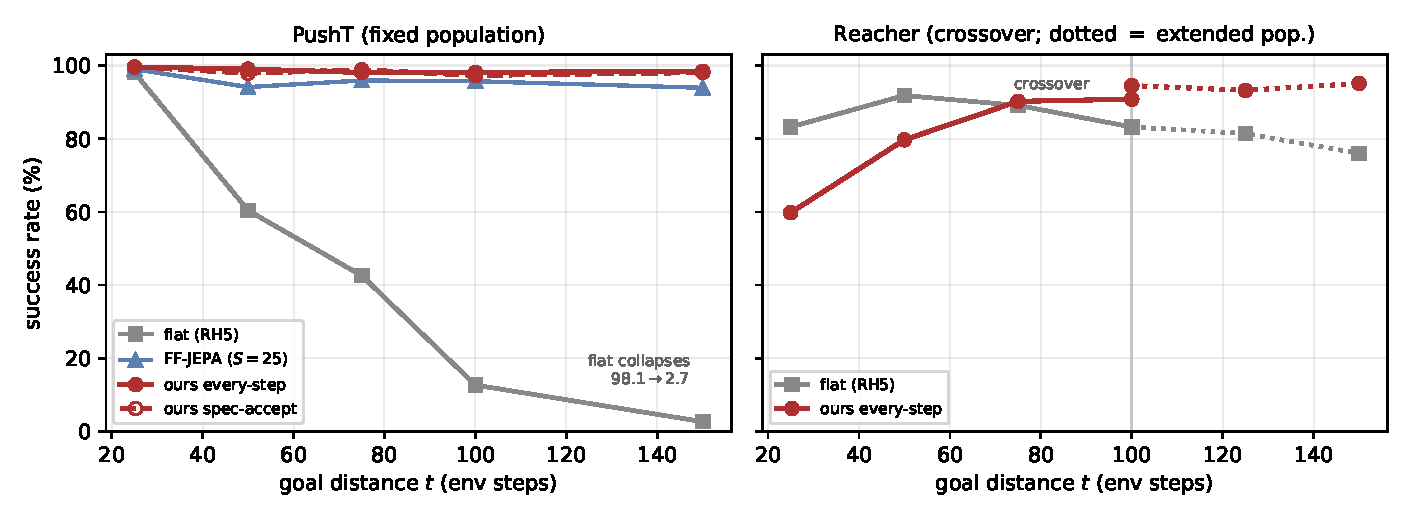
\includegraphics[width=\linewidth]{figs/spine}
\caption{The spine (the paper's centerpiece): success vs.\ goal distance, flat family
vs.\ drafted arms, on the fixed-population sweeps of \Cref{tab:spine}. \textbf{PushT
(left):} flat planning collapses monotonically ($98.1\to2.7$) while every drafted arm
holds ${\sim}98$; spec-accept (open circles) tracks every-step. \textbf{Reacher
(right):} the mechanism as a crossover, flat leads inside the planner's lookahead,
the $S{=}10$ drafter draws level by $t{\approx}75$ and leads thereafter. The two
Reacher populations (solid $=$ max-offset-100 for $t{\le}100$; dotted $=$
max-offset-150 for $t{\ge}100$) are plotted without splicing, both $t{=}100$ values
shown. Cube contributes a single horizon by construction (single-transport task)
and is tabulated in \Cref{tab:cube}; TwoRoom's crossover arc is
\Cref{fig:tworoom-crossover}.}
\label{fig:spine}
\end{figure}

\subsection{One policy at every horizon: certified spec-accept}
\label{sec:results-unified}
The crossover of \Cref{tab:spine} means no fixed arm survives all horizons: flat
collapses at range, drafting pays the decomposition tax up close. The $c^{*}$ arbiter
(\Cref{sec:method-arbiter}) is the closure of that finding, and \Cref{tab:grand} is
the paper's summary view: one policy, no per-cell knowledge, across all three
environments and all eleven environment--horizon cells, above the strongest flat
configuration in every cell, and above or within the declared $\pm1$pp of our own
fixed spec-accept arm everywhere. Everything in it was evaluated the strict way:
fresh, never-analyzed populations (builder seeds disjoint from every analysis
population), success bars frozen in the submission scripts \emph{before} any cell
ran, failures reported as-is. TwoRoom, whose encoder fails the gap precondition
outright, joins as the fourth environment through the same rule with a transplanted
verifier: its window-rule composite ties LeWM's own published protocol and wins
$+15.4$pp beyond the planning window (\Cref{sec:results-heldout}).

\begin{table}[t]
\centering
\small
\setlength{\tabcolsep}{3.2pt}
\caption{\textbf{The headline grid: certified spec-accept beats the strongest flat
configuration in all eleven pre-registered cells.} Confirmation populations, $1024$
episodes/cell; pre-registered verdicts Reacher $4/4$, PushT $5/5$, Cube $+14.0$
against a $+5$ bar. Bold $=$ best in column. Cube contributes one cell by
construction (single-transport task; earlier offsets are vacuous,
\Cref{sec:results-heldout}); arm configurations and populations in
\Cref{tab:spine,tab:protocols}.}
\label{tab:grand}
\begin{tabular}{lccccc|cccc|c}
\toprule
& \multicolumn{5}{c|}{PushT ($t{=}$)} & \multicolumn{4}{c|}{Reacher ($t{=}$)} & Cube \\
& 25 & 50 & 75 & 100 & 150 & 25 & 50 & 100 & 150 & 150 \\
\midrule
LeWM flat (strongest)        & 98.2 & 63.0 & 42.4 & 13.1 & 3.9 & 95.7 & 93.0 & 79.2 & 75.9 & 65.9 \\
spec-accept (fixed arm)      & 99.5 & \ours{98.0} & \ours{98.8} & 98.1 & \ours{98.1} & 57.3 & 78.7 & 88.2 & \ours{91.1} & 76.5 \\
\ours{certified spec-accept (ours)} & \ours{99.7} & 97.5 & 98.1 & \ours{98.5} & \ours{98.1} & \ours{98.7} & \ours{96.3} & \ours{92.3} & 90.1 & \ours{79.9} \\
\midrule
margin vs.\ LeWM flat        & $+1.5$ & $+34.5$ & $+55.7$ & $+85.4$ & $+94.2$ & $+3.0$ & $+3.3$ & $+13.1$ & $+14.3$ & $+14.0$ \\
\bottomrule
\end{tabular}
\end{table} \Cref{tab:unified} gives Reacher, the environment
with the sharpest crossover: certified spec-accept meets or beats the strongest flat
configuration at \textbf{all four horizons}: $4/4$ pre-registered cells on the
declared seeds; pooled over eight seeds the full policy's margins are
$+3.0$/$+3.3$/$+13.1$/$+14.3$pp (SE $0.2$--$0.7$), where every fixed arm loses
somewhere by $15$--$38$pp.
Against our own fixed spec-accept arm it wins outright at $t{\le}100$ and sits
$-1.0$pp behind at $t{=}150$, at the edge of the declared $\pm1$pp band,
persistent across all eight seeds, and reported as such. Routing composition shifts
exactly as the regime map predicts (flat-routed fraction $99\%\to75\%$ over
$t{=}25\to150$), and the certificate's selection is nearly pure: episodes routed to
short-window flat succeed at $96.7$--$100\%$ at \emph{every} horizon and every seed,
including $t{=}150$ where flat's population average is $58.3\%$. Two closures on the
routing rule itself, both computed \emph{exactly} offline from dumped per-episode
outcomes (no new rollouts). \emph{Threshold robustness:} the composite SR is flat
across $\tau\in[0.15,0.40]$ at every horizon (identical to $0.1$pp in most cells;
only $\tau{=}0.10$ under-fires), the router's plateau is wider than the
verifier's, and the shared $\tau{=}0.20$ sits mid-plateau. \emph{Allocation
ceiling:} against the per-episode oracle mix (route each episode to whichever arm
succeeded, the ceiling of any router), the certificate captures $97$--$99\%$ of
the achievable gain at every horizon. \emph{Why both hold, the certificate
separates:} pooled over all horizons and seeds ($2{,}048$ episodes), $c^{*}$ is
bimodal: $70\%$ of episodes sit below $0.15$, where flat succeeds $98.7\%$;
$24\%$ sit above $1.0$, where flat succeeds $17.7\%$ and spec-accept $81.7\%$; and
$6$ episodes in two thousand fall anywhere between. $P(\text{flat succeeds})$ drops
$81$ points across the threshold, and $\tau$ sits in a near-empty valley between
two clean clusters, which is why selection is nearly pure, why any threshold in
$[0.15,0.40]$ makes essentially identical decisions, and why one number can serve
verifier, router, and retirement without per-use tuning.
Finally, the compute-matched control closes the fairness question the arbiter's
overhead raises: doubling flat's CEM samples (a strict upper bound on the measured
$1.58\times$) at $t{\ge}100$ rescues nothing on PushT ($12.7{\to}15.0$ at $t{=}100$;
$3.1{\to}2.9$ at $t{=}150$) and on Reacher buys flat-RH5 $+1$--$2$pp and flat-RH2
$+10$--$12$pp, our frozen prediction (``no material rescue'') was right for three
arms of four and too strong for the under-optimized short window, which we report
as-is. The strongest compute-matched flat configuration reaches $78$--$80$ at
$t{\ge}100$: still ${\sim}12$pp below certified spec-accept, which uses \emph{less}
planning compute than the control. The collapse is a lookahead limit first and an
optimization limit only second.

\begin{table}[h]
\centering
\small
\caption{Certified spec-accept on Reacher (fresh confirmation population, budget
$2t$, $n{=}128$, pooled over 8 seeds $=$ $1024$ episodes/cell; per-cell SE
$0.2$--$0.7$pp; joint criterion). The policy composes the routed episodes: each
episode executed once, under the arm chosen from its start state by $c^{*}$ at frozen
$\tau{=}0.20$. The full policy applies the rule at both scopes
(\Cref{sec:method-arbiter}); the routing-only row is the ablation with mid-episode
retirement disabled, isolating each scope's contribution. Pre-registered bar: the
policy $\ge$ the strongest flat arm at every $t$, scored on the declared seeds
42--45, met $4/4$; the extension seeds 46--49 were declared before their results and
are pooled without selection.}
\label{tab:unified}
\begin{tabular}{lcccc}
\toprule
& $t{=}25$ & $t{=}50$ & $t{=}100$ & $t{=}150$ \\
\midrule
flat, RH$=$2                  & 95.7 & 88.8 & 60.8 & 58.3 \\
flat, RH$=$5                  & 83.0 & 93.0 & 79.2 & 75.9 \\
spec-accept (fixed arm)       & 57.3 & 78.7 & 88.2 & \ours{91.1} \\
routing only (ablation)       & 98.2 & 94.9 & 90.7 & 89.9 \\
\ours{certified spec-accept (full)} & \ours{98.7} & \ours{96.3} & \ours{92.3} & 90.1 \\
\midrule
margin vs.\ strongest flat    & $+3.0$ & $+3.3$ & $+13.1$ & $+14.3$ \\
\bottomrule
\end{tabular}
\end{table}

\textbf{PushT is the do-no-harm test}, pure spec-accept already wins every horizon
there (\Cref{tab:spine}a), so the arbiter's job is to not break it, and the
$c^{*}$-optimism failure mode (mis-routing long-horizon episodes to a flat arm that
scores $2.7\%$) is maximally punished. It does not occur: at $t{\ge}100$ the router
sends $256/256$ episodes to drafting ($c^{*}$ p50 $1.8$--$2.0$, an order of magnitude
above $\tau$), flat branches fire only at $t{\le}50$ where flat is genuinely strong,
and the composite holds $97.1$--$99.8\%$ across $t{=}25\to150$, within the
pre-registered $\pm1$pp of the pure spec spine at every offset ($5/5$ cells), beating
it outright at $t{=}25$ ($99.8$, including a $256/256$ seed) and $t{=}100$. The
full policy (retirement enabled) reads the same ($97.3$--$99.6$, $5/5$). Pooled over four seeds
($1024$ episodes/cell) the picture is unchanged: composite
$99.8/97.0/98.3/98.5/98.1$ across $t{=}25\to150$ vs.\ the pure spec spine's
$99.5/98.0/98.8/98.1/98.1$ (all deltas within $\pm1$pp; at $t{\ge}100$ the composite
\emph{is} the drafting leg, since zero episodes route to flat). On \textbf{Cube} the
arbiter's contribution is reported with the held-out battery
(\Cref{sec:results-heldout}), where it produces the environment's best confirmed
number.

\subsection{Efficiency}
\label{sec:results-eff}

\begin{figure}[h]
\centering
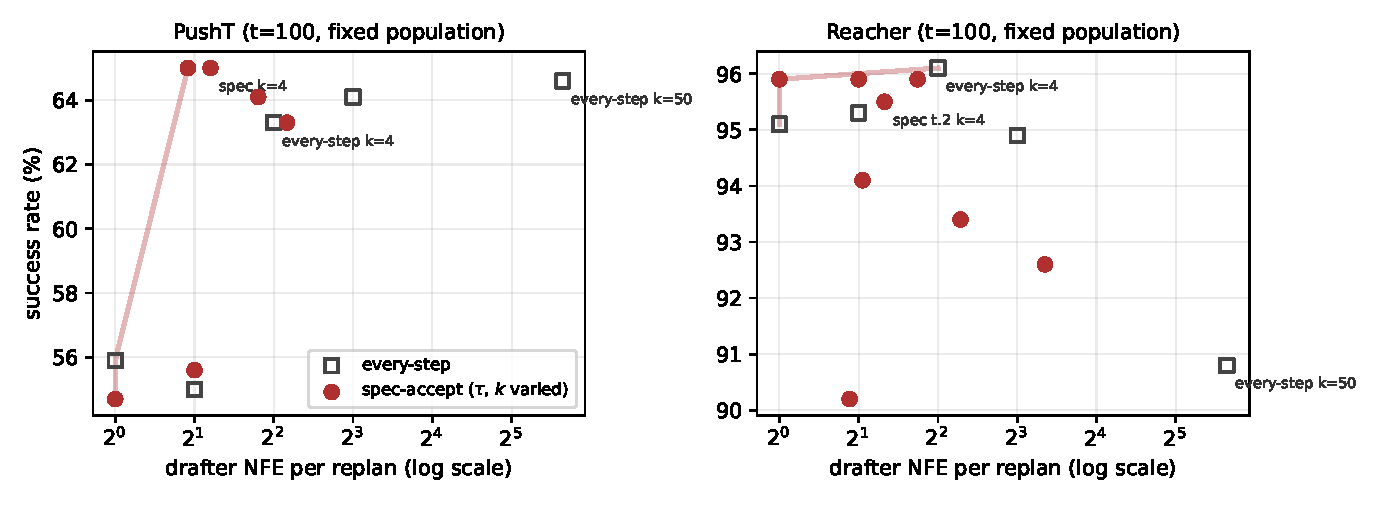
\includegraphics[width=\linewidth]{figs/pareto}
\caption{SR vs.\ drafter compute, every arm on one fixed population per environment
($t{=}100$, $n{=}512$/cell; NFE/replan $=$ call ratio $\times k$). Squares:
every-step drafting across $k$; circles: spec-accept across $\tau$ and $k$; the
frontier is drawn. \textbf{PushT: spec-accept at the frozen config Pareto-dominates}
(higher SR than the $k{=}50$ reference at ${\sim}22\times$ less compute, and than
matched-$k$ every-step at ${\sim}1.7\times$ less). \textbf{Reacher: the frontier is
shared}, cheap every-step drafting is itself strong ($k{=}1$ works), and
spec-accept's marginal factor is ${\sim}1.5\times$ at SR-parity. The $k{\leq}2$ cliff
(PushT, bottom-left) is a consumption-policy artifact, not unusable drafts:
committed blocks at $k{=}2$ recover plateau SR at $1$ NFE/replan
(\Cref{sec:why-verifier}), while $\tau$-verification there falsely rejects
(sampler noise exceeds the floor, \Cref{sec:calib-k}) and inherits every-step's
re-draft churn. The derived $k$ rule keeps the operating point off this cliff.}
\label{fig:pareto}
\end{figure}

At the frozen configuration, spec-accept is SR-neutral or better in every cell of
every regime on both dev environments (call ratios $0.46$--$0.88$), with zero
re-tuning across environments and across goal-free/goal-conditioned drafters
(\Cref{fig:pareto}). Cost, stated as the two factors of \Cref{sec:method-config}:
cheap drafts take the reference from $1500$ to $90$ NFE/episode on their own;
verified consumption removes a further ${\sim}40\%$ of calls at matched $k$, landing
at $1.9$--$2.4$ NFE/replan at the derived configuration.

\paragraph{Why NFE is the right currency.} Measured with CUDA-synced
instrumentation, the drafter is $1.0\%$ of episode wall-clock at $k{=}50$ and $0.4\%$
at the frozen configuration in \emph{this} stack; CEM over an 18M-parameter
dynamics model dominates, and we state that plainly rather than let a wall-clock
number imply otherwise. Drafter NFE is nevertheless the quantity worth optimizing,
for three reasons. First, it is the component that scales: the controller's cost is
fixed by its sample budget and a small dynamics model, while the drafter tier is
where model capacity grows, the same consumption policy applied to a video-scale
drafter inherits the full reduction, and there the drafter \emph{is} the wall-clock.
Second, the factors compose: cheap drafts ($k$) and verified consumption (call ratio)
multiply into any stack with a diffusion proposer, independent of what surrounds it, including stacks whose controller has been distilled or amortized away, where
drafter calls are all that remains. Third, the recipe is wall-clock non-regressive
even here: verification adds no measurable time ($0.4\%$ at $k{=}8$ with or without
spec-accept), and the fine stride it enables runs $12\%$ \emph{faster} end-to-end
than the native configuration at matched protocol. The claim we make is a
drafter-side compute claim, stated with its denominator; the claim we do not make is
an end-to-end latency win on this benchmark.

\paragraph{The arbiter's measured overhead.} The same instrumentation prices the
$c^{*}$ arbiter (PushT $t{=}100$, all-drafting regime, per episode): the derived-$k$
drafter costs $7.9$ms against the controller's $1{,}936$ms ($0.4\%$, drafting is
essentially free at $k{=}3$), and the per-replan retire probe brings certified
spec-accept to $3{,}070$ms, $1.58\times$ the fixed-arm wall-clock, below the $2\times$
bound because the probe plans a shorter window than the policy's own solve. The
asymmetry is the point: at $t{=}25$, where most episodes are certified easy at the
first replan, certified spec-accept completes in $430$ms/episode, cheaper than any
fixed arm, with zero drafter calls on routed episodes by construction. For
reference, the FF-JEPA arms measure $1{,}949$ms ($S{=}10$ loop) and $2{,}449$ms
(native $S{=}25$/RH$=$5) per episode at $2$--$3\%$ drafter share: spec-accept is
wall-clock \emph{ahead} of the published configuration ($-21\%$) at $+2.4$pp SR, and
certified spec-accept costs $1.25\times$ the published configuration for $+2.8$pp. If
the overhead ever matters, the probe admits a knob-free reduction (evaluate $c^{*}$
only at re-draft boundaries, where a solve is being paid for anyway); we report the
conservative every-replan variant throughout.

\Cref{fig:cost} completes the accounting across all three environments ($4$ arms
$\times$ $5$ seeds, measured). Three readings. (i) The overhead is regime-bound: it
appears only where every episode drafts (PushT $t{=}100$: $2.94$ vs.\ spec-accept's
$1.89$s/episode). (ii) On Reacher, certified spec-accept is simultaneously the
\emph{fastest} and the most successful arm ($1.62$s/episode vs.\ flat's $2.11$), routing sends half the episodes to the cheap short window, and successful episodes
terminate early. (iii) Per-episode time is deceptive for failing arms, because failed
episodes burn their whole budget: per \emph{completed task}, flat costs $34$s on
PushT and FF-JEPA $28$s on Cube, against $1.8$--$4.5$s for certified spec-accept
everywhere, the ``cheap'' baseline is the most expensive way to actually finish.

\begin{figure}[h]
\centering
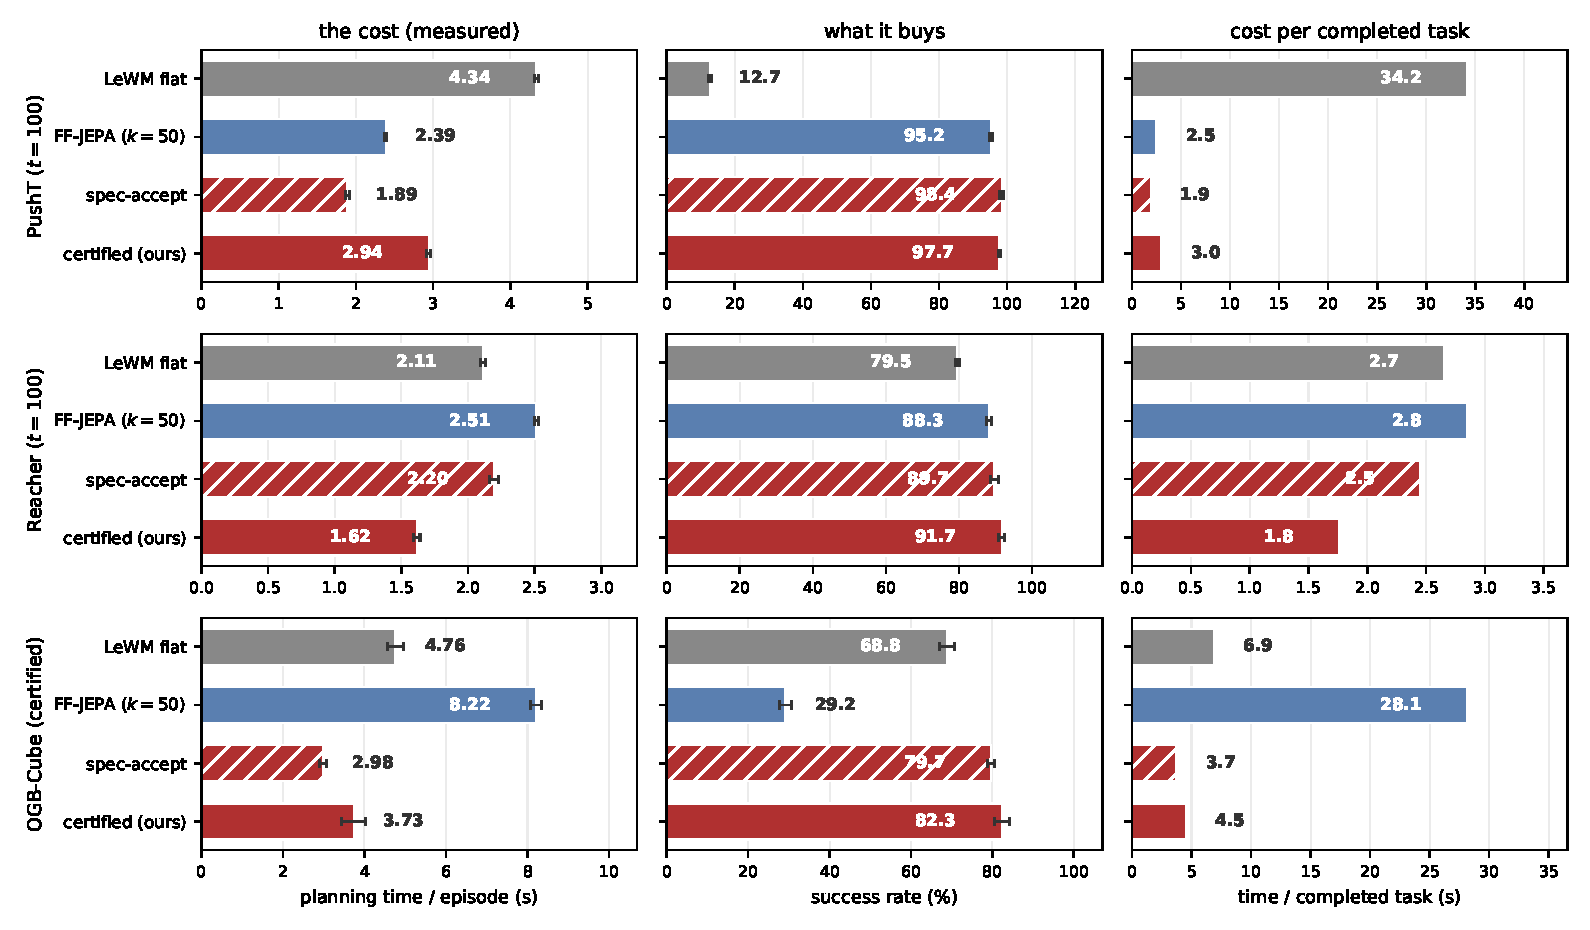
\includegraphics[width=\linewidth]{figs/cost}
\caption{The measured cost story, all three environments ($5$ seeds; two Cube arms
carry $3$--$4$ after node timeouts; error bars $=$ SE). Flat is measured through the
instrumented policy via the lerp-$1.0$ tautology, whose SR reproduces the flat
reference on every environment (the built-in equivalence check); per-episode time
includes early termination on success, the deployment-honest accounting.
\textbf{Left:} the honest overhead, certified spec-accept pays $1.56\times$
spec-accept where everything drafts (PushT), and is outright \emph{fastest} on
Reacher. \textbf{Middle:} what it buys. \textbf{Right:} time per completed task, the failing baselines invert from cheapest to most expensive.}
\label{fig:cost}
\end{figure}

\subsection{Held-out environments}
\label{sec:results-heldout}
% The generalization test the calibration protocol was designed for:
% tau, k frozen; S by the pre-registered rule; no other freedom.

\paragraph{TwoRoom (navigation, bottleneck, unobserved randomized target).}
The structurally hardest case, and the one substrate where the failure sits in the
\emph{planner's own representation} rather than in the method. The per-episode
target is randomized and not rendered in the observation, so goal-\emph{free}
drafting is ill-posed by construction (the sharpest form of the regime rule's
inferability leg, \Cref{sec:why-regime}); that prediction stands. An earlier draft
additionally dismissed goal-\emph{conditioned} drafting on latent-fidelity
grounds; that conclusion traced to two undertrained drafters emitting latents
${\sim}100\times$ off scale and is retracted here, the repaired drafters pass the
same offline fidelity gate as every other environment's (norm ratio $1.01$). What
is actually measured, in order. \textbf{(i) The encoder cannot verify.} LeWM's
TwoRoom latent metric is saturated: consecutive frames sit at rel.\ $L^2$ $0.876$
against a random-pair baseline of $1.456$, and the verification gap is inverted
(equivalence p90 $1.393$ above hop p10 $1.018$), so no threshold separates
arrived from not-arrived; closed loop, verification in this space never fires
(call ratio $0.998$--$1.000$, numerically identical to no verification in every
cell). LeWM's authors independently report Two-Room as their weakest environment
($87$ vs.\ $97$--$100$ for every baseline) and attribute it to a less structured
latent representation; our probe is the direct measurement of that deficit.
\textbf{(ii) The baseline anchors.} Under LeWM's evaluation config verbatim our
flat planner reproduces their published number ($85.3$ mean over three seeds,
their $87$ inside the seed range); the gap to our harder certified protocol is
fully attributed by a cumulative ablation and is dominated by a success-filter
population effect ($+14.6$pp). \textbf{(iii) Verifier modularity recovers the win.} Certifying in a frozen
general-purpose encoder (DINOv2) while the planner keeps consuming LeWM latents
restores a working accept test; a single drafter emits both halves of each
waypoint jointly, so planner and verifier describe the same imagined future. At
the anchored protocol (unfiltered population, LeWM's goal source, flat swept
over replan rate; all bars frozen before any cell ran), certified spec-accept
reaches $57.0$ against flat's $41.7$ at $t{=}75$ over twelve seeds,
$\mathbf{+15.4}$\textbf{pp}, positive on every seed (paired $t{\approx}11$), and
statistically at the ground-truth-waypoint oracle's $56.9$ (twelve seeds both
sides, $t{\approx}0.1$); the margin is
long-horizon only (the oracle itself loses $18$pp to flat at $t{=}25$), making
TwoRoom the third horizon-extension case after PushT and Reacher. Best-of-$k$
drafting scored in the verification space ($k{=}8$, derived offline) passed its
six-seed bar ($+2.9$pp) but shrinks to $+1.8$pp within noise at twelve seeds and
stays an optional add-on outside the headline; verification retains SR within
$0.8$pp of unverified drafting at call ratio $0.94$--$0.97$.
\textbf{(iv) Both sides of the crossover, at their protocol.} At LeWM's own
published evaluation (goal $25$ steps ahead, i.e.\ \emph{inside one planning
window}) our flat replication reads $83.7$ over twelve seeds (their $87$ within
noise), even ground-truth oracle waypoints lose $21$pp, and the certified arm
honestly misses its pre-registered non-inferiority bar ($77.1$; unchanged
pooled at twelve seeds): decomposition
is structurally counterproductive inside the window, at any drafter quality.
Sweeping the goal distance maps the crossover to $t \in [40, 50]$
(\Cref{fig:tworoom-crossover}), just beyond the planning window plus one serving
stride, inside the frozen prediction's band (twelve seeds per arm at $t{=}40$
and $t{=}50$: flat $+3.5$pp at $t{=}40$, spec $+3.4$pp at $t{=}50$; a tie
within seed noise at $t{=}60$; spec $+15.4$pp at
$t{=}75$). Because the goal distance is a known task parameter, the regime rule
composes with a single measured constant, the crossover itself, the same
epistemic status as $\tau$ and $S$: \emph{plan flat up to the measured
crossover ($83.7$, matching LeWM's own game), draft-and-certify beyond it
($57.0$ vs.\ $41.7$)}; the composite never loses to flat at any measured
horizon, the Reacher shape reproduced on a substrate whose planner-space
verification is impossible. Nor is the composite an inference from its
constituent cells: run end-to-end as \emph{one} arm, the driver routing each
task on its known goal distance against the single frozen constant, it
reproduces its branch cell exactly at all five goal distances, passing its
pre-registered per-cell bar with zero deviation. The compute-matched control closes this row as it
does every other: doubling flat's CEM samples (a strict upper bound on the
drafter's overhead) recovers $41.7 \to 47.0$ over twelve seeds, a real
optimization component
reported as-is and stronger than our frozen ``no material rescue'' call, while
certified spec-accept stays $+10.0$pp above the control (paired
$t{\approx}4.9$, $11/12$ seeds)
with less planning compute; the collapse at range is partly optimization,
mostly lookahead. In wall-clock terms, measured through the same instrumented
policy as \Cref{fig:cost}, the near-every-step drafting this substrate forces
(call ratio $0.95$) costs almost nothing: drafter plus DINOv2 verifier add
${\sim}140$ms to a ${\sim}6.9$s episode ($+2\%$; CEM is $94\%$ of wall-clock),
so the $+15.4$pp is effectively free in seconds.
\textbf{(v) Why not the external space everywhere?} Measured, on PushT, whose own
gap is open: one paired drafter, two verifiers, the accept test reading either the
planner-space half ($\tau{=}0.20$, the env's derived threshold) or the DINOv2 half
($\tau{=}0.118$, its criterion floor, derived at runtime). Success is
space-indifferent ($63.5$ vs.\ $62.2$, inside the declared $\pm3$pp band), but the
mechanics are not: the native-space verifier genuinely fires both ways (call ratio
$0.66$, $450$ free advances) while the external one rejects everything it sees
(call ratio $1.00$, zero advances, closed-loop distances sitting above the offline
floor). Transplanting where the native gap is open forfeits the entire call-savings
benefit at equal success, so the rule stands with a measured reason: verify in the
stack's own space when its gap is open, transplant only when it is not.
Three further pre-registered mechanisms failed their bars and are reported as
such: a $3.4\times$-data drafter (null); a feasibility-scored best-of-$k$ whose
stay-put pathology we predicted in advance ($-23$pp, the third demonstration
that offline fidelity does not track closed-loop value, and the first called
before the run); and the $k$-from-sampler-bias derivation, refuted closed-loop
($31.3$ vs.\ $57.0$ at the derived $k{=}2$), with the cause visible in the
probe's own numbers: sample dispersion collapses at low step counts, so the
served drafts mode-average, invisible to a bias-of-means statistic. Certified
serving evidently \emph{requires} sampler diversity, consistent with
best-of-$k$'s positive sign.

\begin{figure}[t]
\centering
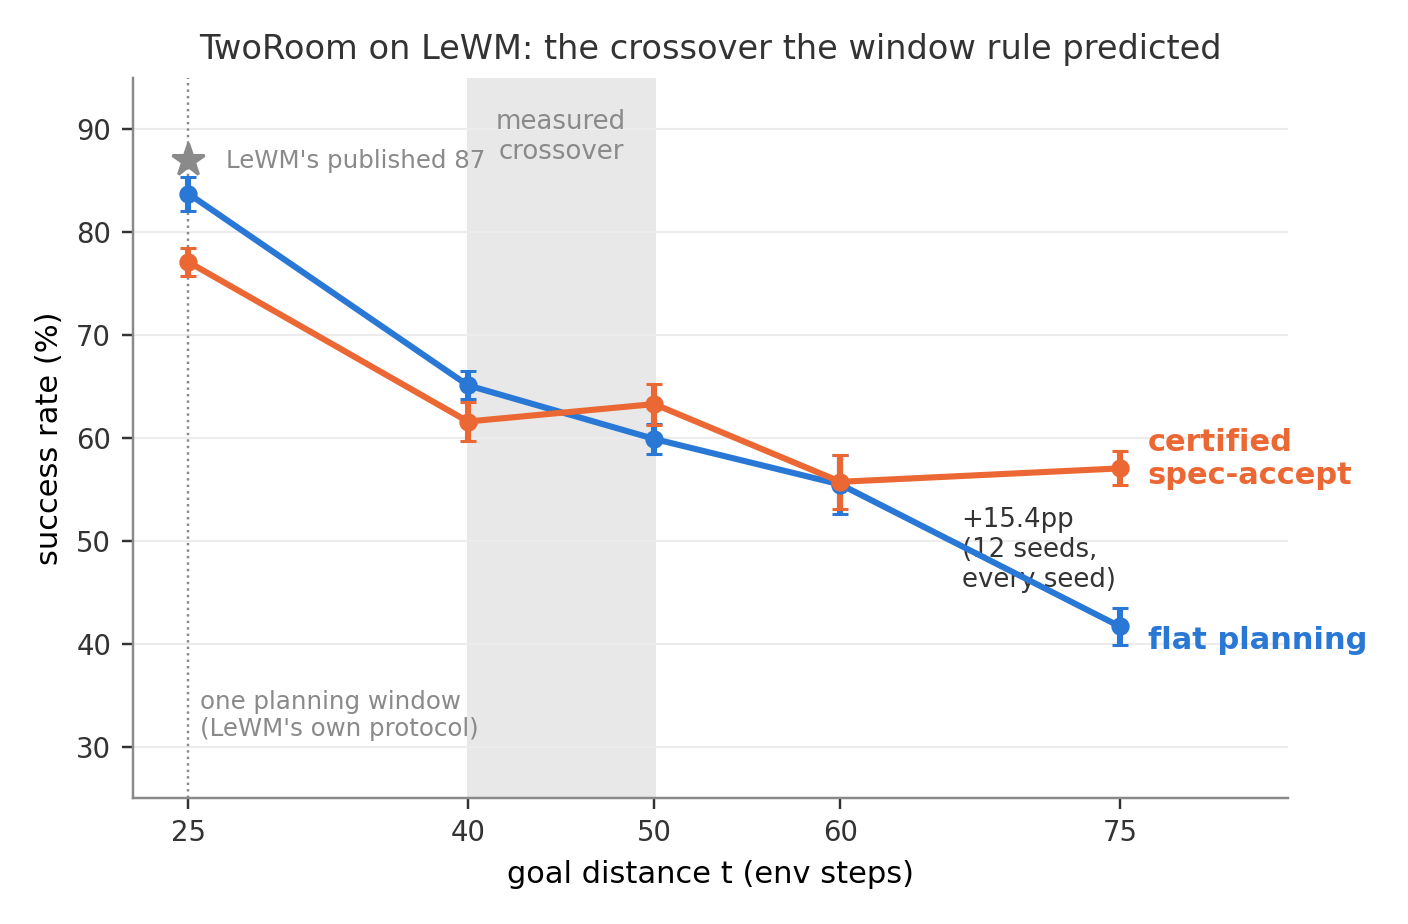
\includegraphics[width=0.72\linewidth]{figures/fig_tworoom_crossover.png}
\caption{\textbf{TwoRoom on LeWM: the crossover the window rule predicted.} Best
flat and best certified spec-accept arm per goal distance (error bars $=$ SE;
$12$ seeds everywhere except the declared $t{=}60$ tie, which stays at $6$; the
$t{=}25$ point is LeWM's
published protocol, star $=$ their Fig.~6 number). The crossover lands in the
shaded band $[40,50]$, inside the frozen prediction; the deployed composite plays
flat left of it and certified spec-accept right of it, and never loses to flat at
any measured horizon.}
\label{fig:tworoom-crossover}
\end{figure}

\paragraph{OGBench-Cube (manipulation): a measured boundary of the threshold rule.}
Cube is the intended out-of-sample test of the \emph{whole} recipe, goal-free
drafter (expert, goal-directed data, the PushT regime), $S{=}10$ zero-shot, and $\tau$
derived from the encoder's criterion floor on an encoder never seen during
calibration. The port reproduces the pipeline (baseline flat planning solves the
single-cube task; encoder and closed loop wire through the benchmark's own $0.04$m
success check), and the $k$-derivation transfers cleanly. The \emph{threshold}
derivation, however, hits a boundary we report rather than paper over: Cube's success
criterion constrains only the cube position, while the encoder observes the whole
scene including the arm. The criterion-floor measurement therefore pairs frames whose
cube matches but whose arm pose does not, inflating the measured floor by
${\sim}10\times$ (p50 $0.97$ vs.\ a normal per-step temporal floor of $0.087$, in line
with PushT's $0.080$). Tightening the equivalence to a \emph{full-scene} match, cube
\emph{and} end-effector, both at the $0.04$m benchmark scale, only partly recovers it
(floor p50 $0.79$, still ${\sim}9\times$ the temporal floor): the encoder retains
substantial visually-salient, task-irrelevant scene variation that no success-based
equivalence pins down. The criterion-floor rule for $\tau$ is thus well-posed only when
the success criterion covers the observed scene; under a \emph{partial}-observation
criterion it is out of scope, and a scope guard (criterion floor within $3\times$ the
temporal floor, else fall back to the transferred default $\tau{=}0.20$) selects the
threshold basis automatically. This is a scope result for the \emph{derivation}, not a
failure of spec-accept, which is threshold-parameterized regardless; the battery ran
the recipe at the transferred-default $\tau$ with the (in-scope) derived $k$, which, applied derive-first to the cube drafter, named $k{=}3$; the closed-loop sweep
run \emph{afterwards} confirms $k{=}3$ as the strongest cell ($81.3$ vs.\ $78.9$ at
$k{=}8$), the derivation rule's second prospective hit.

\paragraph{Cube results: a confirmed win, and one honest miss of the regime map.}
The certified protocol anchors first (flat RH$=$5 reproduces LeWM's published $74\%$
at $71.1$; \Cref{tab:cube}). The regime map's inferability leg then takes its one
loss: \emph{goal-free} drafting fails outright ($33.0$ every-step, $27.3$
spec-accept) despite expert, goal-directed data with a rendered target, the
prediction was that expert data suffices, and it does not; goal-conditioning recovers
$+43$pp on its own ($76.8$, no gating). The failure mechanism is the same overshoot
that bounds short-range Reacher: the drafter, trained on always-in-motion expert
segments, cannot emit ``arrive and stop,'' and the certified task is goal-near
(delivery ${\sim}40$ steps, then a long hold), an arrival gate alone recovers
$+32$pp on the goal-free drafter, and PushT, whose expert episodes \emph{end} at the
goal, is the natural experiment for why it never needed one. With conditioning and
arrival handling the recipe beats flat decisively and approaches the true-waypoint
oracle ($82.4$). All of this then survives the strict test: on eight \emph{fresh}
seeds with the bar frozen in advance ($\ge$ flat $+5$pp), the gated arm confirms at
$+10.5$pp, the exploratory margin ($+10.3$) reproduced on disjoint seeds, and
the $c^{*}$ arbiter (\Cref{sec:method-arbiter}), whose retirement rule replaces the
latent-distance gate, lands \emph{above} it at $79.9$ ($+14.0$ over flat), the
environment's best confirmed number. A decomposition control closes the last
alternative reading: flat at the arbiter's own short window and certified budget
scores only $63.8$, so the win is selection $+$ drafting, not an underrated flat
configuration. One scope nuance is reported rather than smoothed over: on Cube,
$c^{*}$ fires at the first replan on ${\sim}55\%$ of episodes ($c^{*}$ p50
$0.14$--$0.18$) although the physical transport far exceeds the planning window, under a partial-observation criterion the certificate inherits the planner's optimism
toward the goal latent and reads as a per-episode \emph{solvability} signal rather
than literal reachability. The per-episode trace decomposition (pooled, $8$ seeds)
shows that signal is doing real work, the certificate stratifies episodes into a
solvability ladder: episodes retired at the \emph{first} replan succeed at $95.5\%$
($57\%$ of episodes), episodes that draft and then retire on certified arrival at
$75.4\%$ ($33\%$), and the never-retired tail at $9.3\%$ ($10\%$), the genuinely
unsolvable residue, correctly identified by the one signal without any horizon or
task knowledge. We state the instrument's semantics per regime rather than claim
more. Multi-cube (double/triple) remains the genuinely long-horizon manipulation
case and requires that data.

\begin{table}[h]
\centering
\small
\caption{OGBench-Cube, certified protocol (goal offset $150$, budget $300$,
$600$-sample CEM, $n{=}128$/seed; success $=$ cube within $0.04$m). Left: development
seeds. Right: the pre-registered confirmation on eight fresh seeds (bar frozen in
advance: recipe $\ge$ flat $+5$pp, met at $+10.5$ and $+14.0$). Margins are stable
across seed sets; absolutes move with the population and are never compared across
columns.}
\label{tab:cube}
\begin{tabular}{lcc}
\toprule
& dev seeds (4) & fresh seeds (8) \\
\midrule
flat (goal image), RH$=$5                    & 70.9 & 65.9 \\
flat, RH$=$2 (arbiter's window; control)     & ---  & 63.8 \\
goal-free every-step ($k{=}50$)              & 33.0 & --- \\
goal-free spec-accept                        & 27.3 & --- \\
goal-cond.\ spec-accept (no gate)            & 76.8 & --- \\
goal-cond.\ spec-accept $+$ arrival gate, $k{=}3$ & \ours{81.3} & 76.5 \\
certified spec-accept (\Cref{sec:method-arbiter}) & --- & \ours{79.9} \\
\midrule
oracle (true waypoints)                      & 82.4 & --- \\
\bottomrule
\end{tabular}
\end{table}

% ============================================================
\section{Analysis: Why It Works}
\label{sec:why}
% The user-designated killer section. Every claim here is a measured
% mechanism, not narration. Target: a reviewer can reconstruct WHEN the
% method will help on an unseen task, and WHY, from this section alone.

\subsection{Verification is regime-dependent, and the regime is predictable}
\label{sec:why-verifier}
We tested verification against its strongest alternative: \emph{blind commitment}
(consume the next drafted waypoints unconditionally) at matched $k$, on the same
fixed populations. Three regimes, three different answers, one theory.

\textbf{Where drafts track reality, verification is idle, and correctly so.}
In-distribution PushT (expert data), blind commit-2 ties spec-accept at both
anchors ($65.3$ vs.\ $65.0$ at $t{=}100$; $58.1$ vs.\ $58.9$ at $t{=}150$; $k{=}4$)
at call ratio $0.50$ vs.\ spec's $0.53$--$0.63$. A verifier calibrated at the floor
fires only on real divergence; when there is none, it is behaviorally equivalent to
not checking. This tie is a \emph{prediction} of the floor calibration, not a
failure of it.

\textbf{Where drafts genuinely diverge, verification is load-bearing.} On Reacher
(exploratory data; drafts inherit the collection policy's meanders), the verifier
fires constantly (call ratio $0.62$), and removing it costs real success: blind
commitment scores $87.9/89.8$ at $t{=}100/150$ vs.\ spec-accept's $95.5/95.7$, a $+5.9$--$7.6$pp gap. The rejections are re-anchoring events, exactly where the
regime map's data-conditionality leg (\Cref{sec:why-regime}) predicts plans and
reality part ways.

\textbf{Where drafts are \emph{unconverged}, naive verification backfires, as the
floor theory itself explains.} At the PushT $k{\leq}2$ cliff, blind commit-2
scores $63.5$ (plateau quality at $1$ NFE/replan) while spec-accept falls to $55.6$:
with sampler noise far above the floor (\Cref{sec:calib-k}: dispersion $0.65$ vs.\
floor $0.23$), a floor-calibrated $\tau$ rejects everything and inherits
every-step's real failure mode, \emph{churn}, a freshly re-sampled noisy target
every replan that CEM chases. Committed positions of one block are internally
consistent, so commitment beats re-drafting there. The derived $k$ rule keeps the
operating point off this cliff, and we report the cell as the boundary of validity
of floor-calibrated verification rather than hide it.

\textbf{Why not just always commit blindly?} Blind commitment carries a hidden
hyperparameter with its own cliff: depth. Commit-2 is safe on PushT; commit-3 loses
$18$pp there (\Cref{sec:negatives}) and blind commitment loses $6$--$8$pp on Reacher
at the depth its block provides, and blindness has no signal for which regime it
is in. Spec-accept subsumes the whole family ($\tau{\to}0$ is every-step,
$\tau{\to}\infty$ is blind), the measured floor picks the operating point, and the
realized call ratio is a free, per-episode regime diagnostic: ${\approx}0.5$ means
verification is idle insurance; ${<}0.7$ and falling means it is earning its keep.

\paragraph{The churn thesis.} These results and three earlier ones are one
mechanism: \emph{closed-loop control pays for target consistency; re-drafting
injects churn proportional to draft noise; the consumption policy is churn
management}. The cadence-isolation collapse ($-12$pp from re-anchoring against
unchanged targets), the $\gamma$ dose-response (\Cref{sec:why-spread}), the $S{=}5$
anomaly (spec-accept \emph{beating} its own every-step reference by $+5$pp, skipping verified re-drafts of a close target is better control), the $k$-cliff
inversion, and the Reacher blind loss are five independent measurements of the same
quantity from five directions.

\subsection{Drafter stochasticity is load-bearing (dose-response)}
\label{sec:why-spread}
Every operator that collapses drafts toward the conditional mean damages control
despite equal-or-better \emph{offline} fidelity: a deterministic regressor matching
the drafter's offline error loses $4.4$--$11.7$pp closed-loop; a refinement head that
\emph{halves} offline error loses $11$pp. Sweeping the sampler's noise scale $\gamma$
at fixed everything ($\gamma\in\{0,0.25,\ldots,1.5,2\}$, both scales, long-horizon
anchor) unifies these into one curve: SR is non-monotone with the optimum at native
spread, $S{=}25$: $49.0\to53.7\to55.1\to56.1\to\ours{57.9}\to56.1\to28.7\to4.7$
across $\gamma{=}0\to2$; $S{=}10$ traces the same shape with a gentler low side
($56.6$ at $\gamma{=}0$, peak $59.1$--$59.4$ at $\gamma{=}1$--$1.25$, $8.4$ at
$\gamma{=}2$). Closed-loop control pays for conditional spread near the level the
drafter was trained at, in both directions.

\subsection{When drafting pays: the regime map}
\label{sec:why-regime}
Three bounds and one condition, each measured:
\textbf{(i) Decomposition tax.} At short range, ground-truth waypoints tie flat
planning ($84.2$ vs.\ $84.0$, $n{=}512$) and geometrically perfect straight-line
waypoints lose monotonically in hop count ($95.5/70.7/21.9$), decomposition itself
costs when the goal is inside the planner's lookahead; no drafter can beat parity
there.
\textbf{(ii) Necessity at range.} At long range the straight-line oracle fails
($33$--$55\%$ vs.\ the drafter's $94.5$): latent geometry is nonlinear over long
ranges, so the \emph{learned} draft distribution is necessary, not replaceable by
interpolation.
\textbf{(iii) Data conditionality (the $2{\times}2$).} Goal-free drafting works
exactly when the data flows toward goals: on expert PushT data, conditioning changes
nothing ($98.9$ vs.\ $99.4$ short; $60.1$ vs.\ $59.6$ at $t{=}150$, harder
population); on exploratory Reacher data, goal-free drafting is the random-policy
floor ($8.6$--$11.3\%$ vs.\ $60.6$--$95.1\%$ conditioned).
\textbf{(iv) Budget headroom.} Under budget starvation (fixed budget at all
distances) the ordering inverts and flat planning wins (appendix), imperfect
waypoints need slack to pay off.

The operating rule, stated once: \emph{draft when the goal outruns the planning
window, the goal is inferable from data or conditioning, and the budget affords
imperfect waypoints; plan flat otherwise.} TwoRoom and OGBench-Cube
(\Cref{sec:results-heldout}) are the out-of-sample tests of this rule, and the
scorecard is $3.5$ of $4$: PushT (all conditions hold $\to$ drafting wins,
predicted); Reacher (crossover exactly where the goal enters the window, predicted);
TwoRoom (goal not inferable $\to$ goal-\emph{free} drafting fails, predicted;
the certified loop additionally requires a verification space the planner's
encoder cannot supply there, \Cref{sec:results-heldout}); Cube, the honest
half-miss, where the window and budget legs predicted correctly but the
inferability leg did not (expert, goal-directed data with a rendered target was
predicted sufficient for goal-\emph{free} drafting; it is not, and conditioning is
required, \Cref{tab:cube}). We keep the miss in the scorecard: a rule that
survives $3.5/4$ pre-registered predictions with its one failure diagnosed
(arrival is absent from always-in-motion training segments) is worth more than an
unfalsified one. The rule is also no longer only descriptive, the $c^{*}$
arbiter (\Cref{sec:method-arbiter}) is its per-episode operationalization, and
\Cref{sec:results-unified} is the closed-loop test of the rule as a \emph{policy}.

\begin{table}[h]
\centering
\small
\setlength{\tabcolsep}{5pt}
\caption{The regime-map scorecard: the rule's three conditions per environment,
its prediction, and what the batteries measured. Predictions for TwoRoom and Cube
were registered before their runs; the Cube inferability miss is kept in the
scorecard and diagnosed (arrival is absent from always-in-motion training
segments, \Cref{sec:results-heldout}).}
\label{tab:scorecard}
\begin{tabular}{lcccl}
\toprule
env & beyond window? & goal inferable? & headroom? & outcome vs.\ prediction \\
\midrule
PushT   & yes ($t{\ge}50$) & yes (goal-free) & yes & drafting wins, predicted \\
Reacher & at $t{\gtrsim}75$ & conditioned only & yes & crossover at $t{\approx}75$, predicted \\
TwoRoom & yes & \textbf{no} (goal-free) & yes & goal-free fails, predicted; verify in external space \\
Cube    & yes & \emph{miss}: conditioning required & yes & wins once conditioned $+$ arrival \\
\bottomrule
\end{tabular}
\end{table}

% ============================================================
% ============================================================
% NEW SECTIONS (post-freeze program, 2026-07-22 -- 07-27).
% Input from main_v2 just before "Negative Results".
% Every closed number here is from an archived pre-registered run;
% \inflight marks batteries whose bars are frozen and running.
% ============================================================

\section{The Verification Gap: Applicability, Measured in Advance}
\label{sec:instrument}

The criterion floor of \Cref{sec:calib-tau} is half of a more general object. The
accept test must separate two distributions computable from cached latents alone:
\emph{equivalence} distances (states one frame apart, arrived, up to task
tolerance) and \emph{hop} distances (states one subgoal interval apart, did not
move). A workable threshold exists iff the interval
\[
\mathcal{G} \;=\; \bigl[\, \mathrm{equiv}\ p_{90},\;\; \mathrm{hop}\ p_{10} \,\bigr]
\]
is non-empty, and $\tau$ must lie inside it. We call $\mathcal{G}$ the
\textbf{verification gap} and compute it for every substrate this paper touches
(\Cref{fig:gap}), one GPU-pass over cached latents, minutes per environment, no
closed-loop rollouts.

% Figure: the verification-gap instrument across nine substrates (pgfplots).
% Input via % Figure: the verification-gap instrument across nine substrates (pgfplots).
% Input via \input{figures/fig_gap_tikz}. Requires pgfplots (compat>=1.16) and
% \definecolor{gapopen}{HTML}{2A78D6} \definecolor{gapmech}{HTML}{EB6834}
% \definecolor{gapdead}{HTML}{E34948} in the preamble.
\begin{figure}[t]
\centering
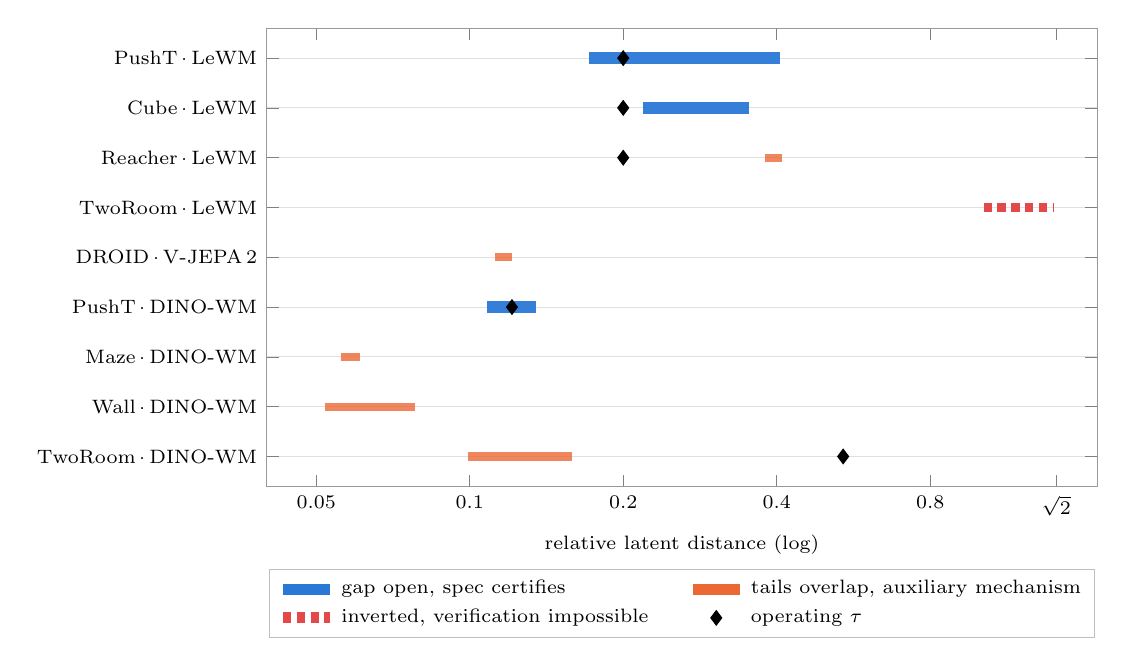
\begin{tikzpicture}
\begin{axis}[
  width=\linewidth, height=7.4cm,
  xmode=log, xmin=0.04, xmax=1.7,
  xtick={0.05,0.1,0.2,0.4,0.8,1.414},
  xticklabels={0.05,0.1,0.2,0.4,0.8,$\sqrt{2}$},
  xlabel={relative latent distance (log)},
  ymin=0.4, ymax=9.6,
  ytick={9,8,7,6,5,4,3,2,1},
  yticklabels={PushT\,·\,LeWM, Cube\,·\,LeWM, Reacher\,·\,LeWM,
               TwoRoom\,·\,LeWM, DROID\,·\,V-JEPA\,2, PushT\,·\,DINO-WM,
               Maze\,·\,DINO-WM, Wall\,·\,DINO-WM, TwoRoom\,·\,DINO-WM},
  y tick label style={font=\scriptsize},
  x tick label style={font=\scriptsize},
  xlabel style={font=\scriptsize},
  axis line style={black!40},
  ymajorgrids, grid style={black!12},
  legend style={font=\scriptsize, at={(0.5,-0.18)}, anchor=north,
                draw=black!25, /tikz/every even column/.append style={column sep=12pt}},
  legend columns=2,
  legend cell align=left,
]
% legend proxies
\addlegendimage{gapopen, line width=4pt}
\addlegendentry{gap open, spec certifies}
\addlegendimage{gapmech, line width=4pt}
\addlegendentry{tails overlap, auxiliary mechanism}
\addlegendimage{gapdead, line width=4pt, densely dashed}
\addlegendentry{inverted, verification impossible}
\addlegendimage{only marks, mark=diamond*, mark size=2.6pt, black}
\addlegendentry{operating $\tau$}

% open gaps [equiv p90 -> hop p10]
\addplot[gapopen, line width=4.5pt, opacity=0.95] coordinates {(0.171,9) (0.406,9)};
\addplot[gapopen, line width=4.5pt, opacity=0.95] coordinates {(0.219,8) (0.353,8)};
\addplot[gapopen, line width=4.5pt, opacity=0.95] coordinates {(0.108,4) (0.135,4)};
% tail overlap (drawn hop p10 -> equiv p90)
\addplot[gapmech, line width=3pt, opacity=0.8] coordinates {(0.379,7) (0.410,7)};
\addplot[gapmech, line width=3pt, opacity=0.8] coordinates {(0.112,5) (0.121,5)};
\addplot[gapmech, line width=3pt, opacity=0.8] coordinates {(0.056,3) (0.061,3)};
\addplot[gapmech, line width=3pt, opacity=0.8] coordinates {(0.052,2) (0.078,2)};
\addplot[gapmech, line width=3pt, opacity=0.8] coordinates {(0.099,1) (0.159,1)};
% inverted (dashed)
\addplot[gapdead, line width=3pt, densely dashed] coordinates {(1.018,6) (1.393,6)};
% taus
\addplot[only marks, mark=diamond*, mark size=2.6pt, black]
  coordinates {(0.20,9) (0.20,8) (0.20,7) (0.121,4) (0.540,1)};
\end{axis}
\end{tikzpicture}
\caption{\textbf{The verification gap across nine substrates.} The verifier must
separate \emph{arrived} (adjacent-frame noise, equiv p90, the criterion floor of
\Cref{sec:calib-tau}) from \emph{did not move} (one subgoal hop, hop p10); the
interval between them is where $\tau$ can operate, computed from cached latents in
minutes. Every closed-loop outcome in this paper matches its row: PushT's in-gap
$\tau$ needed no auxiliary mechanism; Cube's below-gap $\tau$ required the arrival
gate; Reacher's tail overlap required the $c^{*}$ router; TwoRoom-on-LeWM is
inverted at every stride (verification provably cannot operate, even ground-truth
demo waypoints verify $14/113$); DROID's pooled space is degenerate at any $\tau$.
On DINO-WM the instrument ran \emph{before} any closed-loop cell: PushT's gap is
open but the transfer $\tau{=}0.20$ lies above it, so $\tau{=}0.121$ was derived and
frozen; the bottom row shows TwoRoom \emph{cured} of inversion by swapping the
encoder (frozen DINOv2, same pixels), with the learned-lens $\tau$ marked.}
\label{fig:gap}
\end{figure}
. Requires pgfplots (compat>=1.16) and
% \definecolor{gapopen}{HTML}{2A78D6} \definecolor{gapmech}{HTML}{EB6834}
% \definecolor{gapdead}{HTML}{E34948} in the preamble.
\begin{figure}[t]
\centering
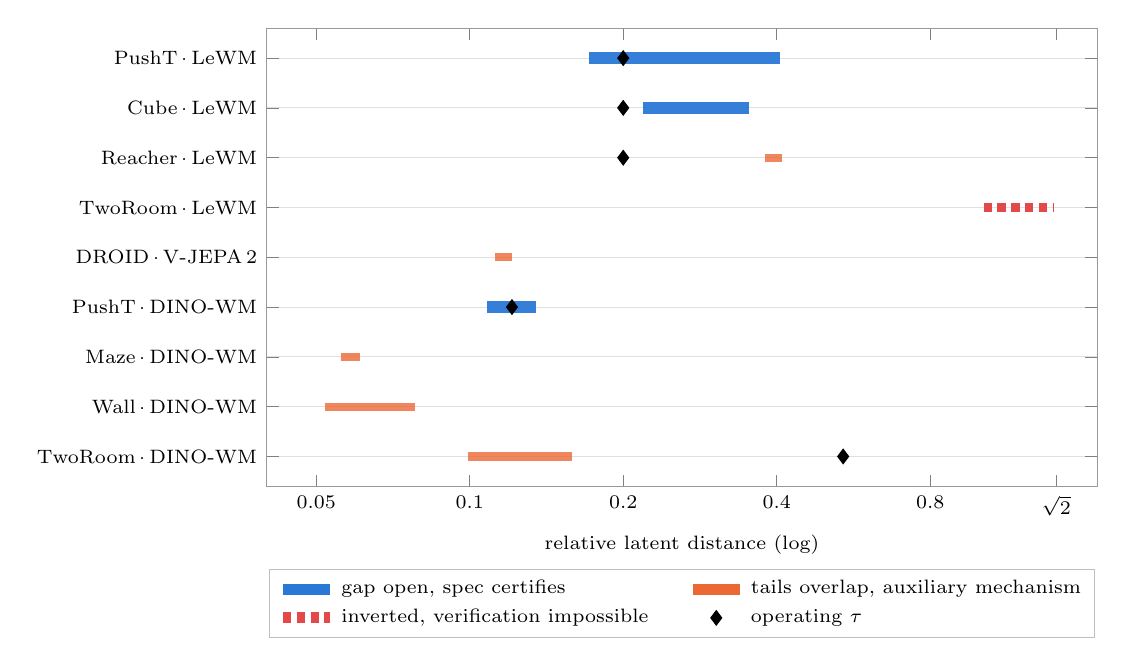
\begin{tikzpicture}
\begin{axis}[
  width=\linewidth, height=7.4cm,
  xmode=log, xmin=0.04, xmax=1.7,
  xtick={0.05,0.1,0.2,0.4,0.8,1.414},
  xticklabels={0.05,0.1,0.2,0.4,0.8,$\sqrt{2}$},
  xlabel={relative latent distance (log)},
  ymin=0.4, ymax=9.6,
  ytick={9,8,7,6,5,4,3,2,1},
  yticklabels={PushT\,·\,LeWM, Cube\,·\,LeWM, Reacher\,·\,LeWM,
               TwoRoom\,·\,LeWM, DROID\,·\,V-JEPA\,2, PushT\,·\,DINO-WM,
               Maze\,·\,DINO-WM, Wall\,·\,DINO-WM, TwoRoom\,·\,DINO-WM},
  y tick label style={font=\scriptsize},
  x tick label style={font=\scriptsize},
  xlabel style={font=\scriptsize},
  axis line style={black!40},
  ymajorgrids, grid style={black!12},
  legend style={font=\scriptsize, at={(0.5,-0.18)}, anchor=north,
                draw=black!25, /tikz/every even column/.append style={column sep=12pt}},
  legend columns=2,
  legend cell align=left,
]
% legend proxies
\addlegendimage{gapopen, line width=4pt}
\addlegendentry{gap open, spec certifies}
\addlegendimage{gapmech, line width=4pt}
\addlegendentry{tails overlap, auxiliary mechanism}
\addlegendimage{gapdead, line width=4pt, densely dashed}
\addlegendentry{inverted, verification impossible}
\addlegendimage{only marks, mark=diamond*, mark size=2.6pt, black}
\addlegendentry{operating $\tau$}

% open gaps [equiv p90 -> hop p10]
\addplot[gapopen, line width=4.5pt, opacity=0.95] coordinates {(0.171,9) (0.406,9)};
\addplot[gapopen, line width=4.5pt, opacity=0.95] coordinates {(0.219,8) (0.353,8)};
\addplot[gapopen, line width=4.5pt, opacity=0.95] coordinates {(0.108,4) (0.135,4)};
% tail overlap (drawn hop p10 -> equiv p90)
\addplot[gapmech, line width=3pt, opacity=0.8] coordinates {(0.379,7) (0.410,7)};
\addplot[gapmech, line width=3pt, opacity=0.8] coordinates {(0.112,5) (0.121,5)};
\addplot[gapmech, line width=3pt, opacity=0.8] coordinates {(0.056,3) (0.061,3)};
\addplot[gapmech, line width=3pt, opacity=0.8] coordinates {(0.052,2) (0.078,2)};
\addplot[gapmech, line width=3pt, opacity=0.8] coordinates {(0.099,1) (0.159,1)};
% inverted (dashed)
\addplot[gapdead, line width=3pt, densely dashed] coordinates {(1.018,6) (1.393,6)};
% taus
\addplot[only marks, mark=diamond*, mark size=2.6pt, black]
  coordinates {(0.20,9) (0.20,8) (0.20,7) (0.121,4) (0.540,1)};
\end{axis}
\end{tikzpicture}
\caption{\textbf{The verification gap across nine substrates.} The verifier must
separate \emph{arrived} (adjacent-frame noise, equiv p90, the criterion floor of
\Cref{sec:calib-tau}) from \emph{did not move} (one subgoal hop, hop p10); the
interval between them is where $\tau$ can operate, computed from cached latents in
minutes. Every closed-loop outcome in this paper matches its row: PushT's in-gap
$\tau$ needed no auxiliary mechanism; Cube's below-gap $\tau$ required the arrival
gate; Reacher's tail overlap required the $c^{*}$ router; TwoRoom-on-LeWM is
inverted at every stride (verification provably cannot operate, even ground-truth
demo waypoints verify $14/113$); DROID's pooled space is degenerate at any $\tau$.
On DINO-WM the instrument ran \emph{before} any closed-loop cell: PushT's gap is
open but the transfer $\tau{=}0.20$ lies above it, so $\tau{=}0.121$ was derived and
frozen; the bottom row shows TwoRoom \emph{cured} of inversion by swapping the
encoder (frozen DINOv2, same pixels), with the learned-lens $\tau$ marked.}
\label{fig:gap}
\end{figure}


\paragraph{One statistic explains every outcome.} PushT's $\tau{=}0.20$ sits inside
its gap $[0.171, 0.406]$: pure spec-accept wins with no auxiliary mechanism
(\Cref{tab:grand}). Cube's gap $[0.219, 0.353]$ sits just \emph{above} the transfer
$\tau$: slight over-rejection, and indeed Cube required the arrival gate. Reacher's
bulks separate $4\times$ but the tails overlap (equiv $p_{90}$ $0.410$ vs.\ hop
$p_{10}$ $0.379$): a noisy verifier, and indeed Reacher required the per-episode
$c^{*}$ router. TwoRoom-on-LeWM is \emph{inverted at every stride}: adjacent
frames read $0.88$ median while unrelated episodes read ${\approx}\sqrt{2}$, the
encoder assigning near-orthogonal codes to distinct positions. No threshold
exists, and the behavioral evidence agrees: a verified oracle serving waypoints the
demonstrator \emph{physically visited} accepted $14/113$ of them. DROID's pooled
space opens no gap at any stride: verification runs degenerate-accept, which is the
honest scope of the scale transplant (\Cref{sec:generality-scale}).

\paragraph{Prescription has a measured boundary.} The instrument's applicability
claim (gap exists $\Rightarrow$ a $\tau$ exists; inverted $\Rightarrow$ verification
cannot operate) is distinct from a stronger prescription we tested and reject: that
the gap \emph{midpoint} is the right $\tau$ and can replace an auxiliary mechanism.
Pre-registered on Cube (8 seeds, gate off, $\tau{=}0.286$ at the midpoint): mechanics
moved as predicted (acceptances ${\sim}3\times$) but SR \emph{fell} to $74.6$ against
a $\ge 78.0$ bar with seed variance tripled: the gate's margin is arrival
protection, not threshold mis-calibration. We therefore claim applicability and
$\tau$-existence, not $\tau$-optimality.

\paragraph{Prospective record.} Three predictions were frozen before their tests and
confirmed: (i) a learned attentive readout cannot open DROID's pooled gap with
$8\times$ data (still closed, width $-0.107$); (ii) $20\times$ data does not repair
the DROID drafter's latent fidelity (no-op ratio $0.39$--$0.48\times$, vs.\ v1's
$0.53$--$0.63\times$); (iii) nor its planning value (paired against v1 across three
budgets: $+0.015/-0.053/+0.074$, all CIs straddling zero). Six further predictions
were frozen before their tests on DINO-WM; their verdicts, including the ones the
serving fault left unresolvable, are reported in \Cref{sec:generality-dinowm}.

\paragraph{When the gap is closed but recoverable: the lens.} Where bulks separate
but tails overlap, a small time-contrastive readout (verifier-side only; world model
and planner untouched) can reopen the interval on held-out episodes: Reacher
$-0.039 \to +0.031$ (derived $\tau{=}0.309$), and on the DINO-WM substrates below,
Maze $-0.006 \to +0.167$, Wall $-0.012 \to +0.146$, TwoRoom-on-DINOv2
$-0.055 \to +0.229$. Two honest boundaries: DROID's pooled space resists the lens at
any tested data scale (information absent from the readout, not mis-read), and an
open lens gap is an \emph{offline} statement: closed-loop, the Reacher lens
traded short-horizon SR ($-4.5$/$-2.5$pp at $t{=}25/50$) for verification
efficiency (call ratio $0.63 \to 0.55$); its closed-loop value is tested
pre-registered on Wall below.

% ============================================================
\section{Generality: A Second Architecture and a Scale Transplant}
\label{sec:generality}

The results of \Cref{sec:results} live on one stack. This section transplants the
method twice, to a second full planning architecture where closed-loop success is
measurable, and to a $55\times$ larger world model where it is not, and lets the
instrument of \Cref{sec:instrument} make its predictions \emph{first}.

\subsection{DINO-WM: derive-first on an architecture adopted mid-project}
\label{sec:generality-dinowm}

DINO-WM \citep{dinowm} plans with MPC-CEM over frozen DINOv2 patch features, a
task-agnostic encoder, unlike LeWM's task-trained one, and therefore the harder
test of the gap's portability. We reproduce its released PushT protocol as the
anchor (flat success $86\%$ at $n{=}50$, seed $99$, vs.\ the paper's $90\%$; our run
caps MPC at the environment's 300-step episode budget), then run the instrument
before any spec-accept cell: PushT's gap is \emph{open} at the natural hop but the
LeWM-transfer $\tau{=}0.20$ sits \emph{above} it, the instrument's first
$\tau$-mis-calibration call; so $\tau{=}0.121$ is derived and the following are
frozen (\texttt{docs/dinowm\_prereg.md}) before execution: \textbf{P1} certified
spec-accept at $\tau{=}0.121$ within $2$pp of flat; \textbf{P2} $\tau{=}0.20$ runs
degenerate-accept; \textbf{P3} Maze/Wall (tail-overlap rows) underperform at any
fixed $\tau$; \textbf{P4} Wall recovers under the lens verifier; \textbf{P5} at
$\mathrm{goal}_H{=}15$, where the drafted block spans the goal distance exactly, the
spec-vs-flat margin improves on its short-horizon value. The transplanted drafter is
the first in this program to beat the no-op reference on a video-feature substrate
(no-op ratio $1.11/1.22/1.31\times$ at block positions $1/2/3$).

Verdicts, reported exactly as they fell. \textbf{P3 confirmed}, the cleanest
prospective hit in the program: Wall at the fixed transfer $\tau$ scores $0.685$
against flat's $1.00$, a $31$pp underperformance the instrument called before the
run. \textbf{P4 unavailable}: the Wall lens never opened a gap at the serving hop,
so no $\tau$ could be derived and the arm was not run, reported rather than
improvised. \textbf{P1, P2, and P5 are confounded and remain open}: across three
independent batteries the flat arms are healthy ($0.82$--$0.88$) while every
spec-accept arm scores near zero with one signature (the drafter passes its offline
gates and beats the no-op reference, yet served waypoints produce no progress),
which indicates an unresolved fault in our DINO-WM serving integration rather than
a verdict on the predictions; we decline to claim them in either direction, and the
predictions stay frozen. Point-maze remains prediction-only (its environment
requires mujoco-py + d4rl).

\subsection{TwoRoom: the scope condition is an encoder property, and repairable}
\label{sec:generality-tworoom}

TwoRoom-on-LeWM is this paper's cleanest impossibility (\Cref{sec:instrument}):
inverted gap, verifier rejecting reality itself, ground-truth waypoints
\emph{halving} flat's success because planning optimizes the same broken metric. The
instrument localizes the failure to the encoder, which makes a causal test
available: push the \emph{same pixels} through frozen DINOv2. The saturation cures:
adjacent-frame distance drops $0.876 \to 0.081$, hops and cross-episode
distances scale properly again, and the substrate lands in the recoverable
tail-overlap class, where the lens opens a usable gap ($+0.229$, derived
$\tau{=}0.540$). The scope condition is not ``TwoRoom is hard'': it is a measurable
property of the encoder's metric, diagnosed in advance, and repaired by a component
swap the instrument itself prescribed.

The closed-loop completion on this substrate (a DINO-WM world model trained on
TwoRoom, drafted arm under the lens verifier) was cut at the program's
pre-declared deadline before its evaluation harness was complete; the encoder-swap
cure above is the measured claim, and the closed-loop arm remains a frozen
prediction. The LeWM-side closed loop, however, did complete
(\Cref{sec:results-heldout}): certifying TwoRoom in frozen DINOv2 while the
planner consumes LeWM latents recovers $+15.4$pp at range, the same
component-swap prescription executed on the verifier alone.

\subsection{V-JEPA 2: what transfers at $55\times$ scale, and what cannot be known offline}
\label{sec:generality-scale}

Transplanted to V-JEPA~2's 1B action-conditioned model (token-grid targets served to
the upstream CEM unmodified), the \emph{mechanism} carries: the certified source runs
end-to-end, and the verifier constant transfers ($\tau{=}0.20$ against measured
single-replan floors of $0.06$--$0.10$). Three things do not, and we report them as
the scale boundary. The planner certificate $c^{*}$ carries no discriminative signal
on this substrate (three independent measurements; a router built on it routes
$0/36$ anchors to flat). The drafter is not rescued by data ($20\times$: predictions
(ii)--(iii) above). And planning \emph{quality} cannot be honestly adjudicated
offline at all: there is no simulator for a real-robot DROID model, in-model scoring
is circular (the model grades plans that may exploit its own errors), and the
demonstration-agreement instrument fails its own sanity checks at $n{=}36$ paired
anchors (flat's agreement ${\approx}0$ and not improving with $16\times$ budget; a
straight-line interpolation outscoring both planners). An exploratory
$15\times$-compute result did not survive this powered pre-registered replication
and is retired accordingly; closed-loop evaluation at scale is future work requiring
hardware, not more offline instruments.

\paragraph{Concurrent work.} SAGE \citep{sage} (July 2026) independently reports that
drafted subgoal latents repair long-horizon myopia on LeWM, converging evidence
for the premise, but consumes its drafts open-loop: no reality-verification, no
applicability instrument, one architecture. TRM \citep{trm} repairs latent-metric
failures with reachability-based metrics, the training-time complement to our
verifier-side lens; its LeWM-vs-PLDM TwoRoom comparison independently supports the
encoder-property reading of \Cref{sec:generality-tworoom}. Our contribution remains
the certificate and the instrument: \emph{when} a drafted plan can be trusted, and
\emph{whether} a given stack can support the trust test at all.


% ============================================================
\section{Negative Results and Ablations}
\label{sec:negatives}
Every alternative we measured loses to the recipe, and each loss confirms one of the
two mechanisms of \Cref{sec:why}. \emph{Spread is load-bearing:} refinement head
$-11$pp, blind commit-3 $-18$pp, learned-confidence adaptive commit worse than blind,
deterministic regressor $-4.4$ to $-11.7$pp at matched offline fidelity. \emph{The
verifier must be reality, not a heuristic:} a goal-gated variant (serve the goal
image whenever a waypoint fails a latent goal-progress test, one greedy attempt to
automate the regime rule inside the verifier) collapses the Reacher long-horizon
advantage from $94.5/93.9$ back toward the flat baseline ($82.8$ at $t{=}100$, $80.1$
at $t{=}150$; call ratio ${\sim}0.8$), while remaining harmless where drafting had no
edge anyway ($91.6$ at $t{=}25$). The matched-$k$ blind-commitment cells of
\Cref{sec:why-verifier} complete the picture: blindness is not uniformly wrong, it ties where verification is idle, but it fails unsignaled in both directions
(depth-3 on PushT, any depth on Reacher), which is precisely what a measured
threshold buys over a commitment ladder.

\begin{table}[h]
\centering
\small
\setlength{\tabcolsep}{5pt}
\caption{Negative results, every alternative to the recipe, grouped by the mechanism
each confirms (controlled protocols; \degc{20} / joint criterion). Every operator that
narrows the drafter's conditional spread toward its mean, or replaces the reality
verifier with a proxy, loses, despite equal-or-better \emph{offline} fidelity in the
spread rows. $\Delta$ is versus that block's reference. The goal-gated row is
diagnosed, not merely reported: latent distance to the goal saturates beyond one hop
(\Cref{sec:calib-tau}), so the gate fires on noise at range and collapses the
long-horizon advantage, while the \emph{same} gating idea, applied where distances
are informative (arrival on Cube, \Cref{tab:cube}), recovers $+32$pp. The $c^{*}$
arbiter (\Cref{sec:method-arbiter}) replaces the saturating instrument with the
planner's certificate and recovers both regimes at once
(\Cref{sec:results-unified}).}
\label{tab:negatives}
\begin{tabular}{llcc}
\toprule
mechanism & arm & SR & $\Delta$ \\
\midrule
\multirow{5}{*}{\shortstack[l]{spread is\\load-bearing}}
 & GDM every-step (PushT reference)          & 91.9 & --- \\
 & $+$ refinement head (halves offline err.) & 81.1 & $-10.8$ \\
 & $+$ blind commit-3                         & 73.8 & $-18.1$ \\
 & $+$ learned-confidence adaptive commit     & 64.5 & $-27.4$ \\
 & deterministic regressor (matched offline)  & \multicolumn{2}{c}{$-4.4$ to $-11.7$} \\
\midrule
\multirow{2}{*}{\shortstack[l]{verify vs.\\reality}}
 & spec-accept (Reacher long, reference)      & 94.5\,/\,93.9 & --- \\
 & goal-gated verifier (learned proxy)        & 82.8\,/\,80.1 & $-11.7$\,/\,$-13.8$ \\
\midrule
\multirow{2}{*}{\shortstack[l]{blindness\\unsignaled}}
 & blind commit-2, PushT (verify idle here)   & 65.3 & $+0.3$ \\
 & blind commit-3, Reacher (any depth)        & 87.9\,/\,89.8 & $-6.6$\,/\,$-5.9$ \\
\bottomrule
\end{tabular}
\end{table}

\Cref{tab:negatives} collects them. The dose-response of \Cref{sec:why-spread} is the
continuous version of the top block, and the $\gamma$-sweep's interior optimum at
native spread is what makes ``narrow the spread'' predict a loss in both directions.

% ============================================================
\section{Discussion and Limitations}
\label{sec:discussion}
\textbf{What the story is.} Closed-loop success in this planner is governed by matching
the control loop to the subgoal scale and by consuming drafts only while reality
confirms them; the drafter's conditional \emph{spread} is load-bearing, and the two
consumption knobs are measured, not tuned. The efficiency win is orthogonal to the
success story: reality is a free verifier.

\textbf{Limitations.} (i) FF-JEPA is a preliminary paper with no released code; our
``faithful'' configuration is a principled reconstruction where the paper is silent,
certified by closed-loop anchor cells (\Cref{app:repro}), not a verified match on every
axis. (ii) The derivation of $\tau$ and $k$ is validated retrospectively on two
development environments plus \emph{two} prospective confirmations; PushT's
$k{=}3$ (named by the measurement before the sweep ever ran it) and Cube's
derive-first $k{=}3$ (named from the held-out drafter's dispersion, later confirmed
the sweep's strongest cell); the $\tau$ rule, by contrast, met its measured scope
boundary on Cube (\Cref{sec:results-heldout}) and fell back to the transferred
default there, the derivation program's one honest asymmetry. (iii) The criterion-floor rule
for $\tau$ has a \emph{measured} scope boundary: it is well-posed only when the
benchmark's success criterion covers the observed scene, and inflates under
partial-observation criteria (Cube, \Cref{sec:results-heldout}), where a full-scene or
temporal-floor threshold basis is required. (iv) The value of drafting itself is
\emph{conditional}, not universal: it requires goals beyond the planning window, budget
headroom, and goal-inferable data (the regime map, \Cref{sec:why-regime}); on tasks
inside the planner's lookahead even ground-truth waypoints do not beat flat planning.
(v) The \degc{20}/\degc{5} criterion mapping for the paper's own cells is inferred from
empirical alignment, not stated by the paper; every cross-paper comparison is marked
with the side it is valid on. (vi) The compute claim is a drafter-side NFE claim stated
with its denominator, not an end-to-end latency win on this CEM-dominated stack; its
force is in stacks where the drafter dominates (\Cref{sec:results-eff}). (vii)
Horizon-sweep populations are eligibility-defined and never spliced across offsets or
populations; success-filtered and unfiltered populations give the same qualitative
story at different absolute levels and are reported separately. (viii) The
arbiter's routing guarantee is \emph{empirical}, not structural: $c^{*}$ is the
planner's self-assessment, well-calibrated on these three world models (selection
purity $96$--$100\%$) but inheriting any mis-calibration of the world model itself;
failure degrades softly to the routed parent arm. Relatedly, certified spec-accept
\emph{allocates} capability rather than creating it, it is upper-bounded by the
per-episode oracle mix of its parents (${\approx}94.5$ at Reacher $t{=}150$, where it
reaches $90$--$92$), and on partial-observation criteria its certificate reads as
per-episode solvability rather than literal reachability
(\Cref{sec:results-heldout}). Its measured overhead is $1.58\times$ fixed-arm
wall-clock on drafting episodes and below-baseline on certified-easy ones
(\Cref{sec:results-eff}).

% ============================================================
\section{Conclusion}
\label{sec:conclusion}
A hierarchical latent planner can trust a drafted plan exactly as long as reality
confirms it, and the threshold for ``confirms'' is a measured property of the
encoder, not a hyperparameter. Certified spec-accept turns that observation into one
policy that wins all eleven pre-registered cells across three environments at
$1.9$--$2.4$ drafter evaluations per replan, with both constants derived offline and
confirmed prospectively. The verification gap makes the method's precondition itself
measurable in advance, and its predictions have held on substrates adopted after
the rule was frozen; when the precondition fails outright, the repair is modular
rather than architectural, as Two-Room shows: certify in a frozen external encoder,
compose with the window rule, and the stack's weakest published result becomes a
certified $+15.4$pp win at range without retraining the world model. Nothing in the
recipe is substrate-specific: any world model that plans by rollout can grade its
own homework the same way, and the open frontier is scale, where the drafter tier
rather than the controller is the wall-clock.

% ============================================================
\appendix
\section{Faithful Reproduction and Audit}
\label{app:repro}
Every number in this paper is produced by a pipeline rebuilt end-to-end from public
assets on independent hardware. Faithfulness is over-determined. A from-scratch rebuild
of the dense training set reproduces the original training population to the episode
($9{,}094$) and the optimizer to the iteration ($171{,}940$); the retrained $S{=}25$
drafter reproduces the reference offline-fidelity anchor to four decimals ($0.1593$
vs.\ $0.1593$ at $m{+}1$); and the closed-loop anchor cells reproduce the original
system within noise (baseline $94.6$ / oracle $92.6$ / $S{=}25$ $94.8$ / $S{=}10$
$99.4$ \degc{20}, against the box-era $93.4/93.4/95.3/98.4$). Offline drafter
diagnostics are not comparable across dense-file rebuilds; the closed-loop anchors are
the arbiter.

\paragraph{The \degc{20}/\degc{5} criterion.} FF-JEPA's prose states a \degc{5} angular
tolerance, but the environment's shipped evaluation code enforces \degc{20}; the oracle
(true goal, exact pipeline) reaches only ${\sim}84$--$86\%$ at literal \degc{5} even
under matched-population filtering, making a genuine $96\%$ at \degc{5} for a
\emph{sampled}-subgoal method implausible. We treat \degc{20} as the operative
criterion (it is what the code enforces and what every published number matches) and
\degc{5} as a strict precision criterion, reporting both throughout.

\paragraph{Protocols.} \emph{Paper protocol}: $n{=}256$, paper-matched sampling
(reproduction, random-init, and the FF-JEPA-config comparison rows). \emph{Controlled
protocol}: fixed held-out episodes, budget $2t$, block-only criterion, CEM seeds
matched byte-for-byte across arms so within-table deltas are exact treatment effects;
per-arm $\mathrm{SE}\approx1.7$pp (4 seeds) / $0.9$pp (8 seeds). Horizon sweeps use one
fixed episode population per environment, identical episodes at every offset; the two
Reacher populations (max-offset-100 / -150) and the PushT success-filtered /
unfiltered populations are never spliced. Confirmation populations use fresh builder
seeds disjoint from every analysis population ($777$ for gate v3, $888$ for the v4
exploratory run, $999$ for the v4 confirm); seed extensions to $1024$
episodes/cell were declared before their results and pooled without selection.

\begin{table}[h]
\centering
\small
\setlength{\tabcolsep}{4pt}
\caption{Per-environment protocols (every closed-loop cell in the paper).}
\label{tab:protocols}
\begin{tabular}{lp{3.2cm}p{3.4cm}p{5.4cm}}
\toprule
& PushT & Reacher & OGBench-Cube (single) \\
\midrule
success criterion & block pose, \degc{20} (\degc{5} strict) & all joints within $0.05$\,rad & cube within $0.04$\,m of target \\
episodes/cell & $256\times4$ seeds & $128\times8$ seeds & $128\times8$ seeds (confirm) \\
budget & $2t$ & $2t$ & $300$ at offset $150$; $600$-sample CEM \\
populations & success-filtered $+$ unfiltered fixed & max-offset-$100$/$150$ $+$ confirm (seed $999$) & holdout episodes ${\ge}8000$, per-seed sampling \\
drafter & goal-free, $S{=}10$ & goal-cond., $S{=}10$ & goal-cond., $S{=}10$ \\
$k$ / $\tau$ & $3$ (derived) / $0.20$ (derived) & $8$ (rule: any) / $0.20$ (in-band) & $3$ (derive-first) / $0.20$ (transferred; scope guard) \\
\bottomrule
\end{tabular}
\end{table}

\section{Controls and Full Grids}
\label{app:controls}
The following controls are summarized in the main text and reported in full here (all
exist in the run logs; provenance in the supplementary).
\begin{itemize}[itemsep=1pt,topsep=2pt]
\item \textbf{Cadence isolation} (\Cref{sec:method-scale}): re-anchoring every $5$ steps
against \emph{unchanged} $25$-step targets collapses SR to $78.6/77.8$ ($-12.5$pp), the mechanism is scale matching, not replan frequency.
\item \textbf{Full $\tau{\times}k$ grid} behind \Cref{fig:pareto}, both environments,
with call ratios; the frozen cell and the $k$-cliff are read off it.
\item \textbf{Replan-rate (RH) sweeps} for the flat baseline, both environments: RH is a
brittle short-vs-long trade-off (Reacher RH$1/2/5$ at $t{=}25$: $91.6/95.7/83.2$; at
$t{=}150$: $46.1/62.3/76.0$), so every comparison anchors to the strongest flat
configuration per cell; no RH rescues flat planning from the horizon collapse.
\item \textbf{Fixed-population horizon tables} at both success-filtered and unfiltered
populations (PushT), reported separately, same qualitative story at different absolute
levels.
\item \textbf{VLWM fixed-budget-50 cross-paper cell}: budget starvation reproduces the
published collapse and inverts the drafting/flat ordering (imperfect waypoints need
budget headroom); cited as ``same budget regime,'' not a like-for-like win.
\item \textbf{Failure anatomy} ($S{=}10$, 8 seeds): $18$ failures in $496$ episodes, all
tolerance-boundary near-misses (final distance within the success distribution's 95th
percentile); zero unreachable-subgoal, divergence, or stuck episodes; FF-JEPA's own
reported failure mode is eliminated at fine scale.
\end{itemize}

\bibliography{references}
\bibliographystyle{iclr2026_conference}

\end{document}
